%%
%% Computers & Industrial Engineering -- Elsevier CAS template (cas-sc).
%% Bibliography style: cas-model2-names (author-year).
%%
%% Copyright 2019-2024 Elsevier Ltd. Template distributed under the
%% LaTeX Project Public License (see http://www.latex-project.org/lppl.txt).
%%

\PassOptionsToPackage{hyperfootnotes=false}{hyperref}
\documentclass[a4paper,fleqn]{cas-sc}
%\documentclass[preprint,12pt]{elsarticle}
% If the front matter runs over more than one page, use the longmktitle option in Overleaf if supported by the installed CAS bundle.
%\documentclass[a4paper,fleqn,longmktitle]{cas-sc}

\usepackage[authoryear,longnamesfirst]{natbib}

\usepackage{amsmath,amssymb}
\usepackage{booktabs}
\usepackage{multirow}
\usepackage{array}
\usepackage{xcolor}
\usepackage{csvsimple}
\usepackage{graphicx}
\usepackage{subcaption}
\usepackage{siunitx}
\usepackage[section]{placeins}
\usepackage{float}
\usepackage{colortbl}
\usepackage{pdftexcmds}
%\usepackage[authoryear]{natbib}
% Row highlighting for the Pareto-front table: \hl is placed in every cell and
% is set per row to either \hlon (shaded) or \relax (plain).
\newcommand{\hlon}{\cellcolor{gray!20}}
\let\hl\relax
\makeatletter
\newcommand{\IfSelectedRow}[1]{%
  \global\@tempswafalse
  \@for\@selidx:=1,2,3\do{%
    \@ifundefined{selrow\@selidx}{}{%
      \ifnum\pdf@strcmp{#1}{\csname selrow\@selidx\endcsname}=\z@ \global\@tempswatrue\fi}}%
  \if@tempswa\expandafter\@firstoftwo\else\expandafter\@secondoftwo\fi}
\makeatother
% Loosen LaTeX float parameters so near-full-page figures do not
% cascade to the end of the document. Defaults are too tight for a
% figure-dense manuscript.
\renewcommand{\topfraction}{0.9}
\renewcommand{\bottomfraction}{0.9}
\renewcommand{\textfraction}{0.05}
\renewcommand{\floatpagefraction}{0.7}
\setcounter{topnumber}{4}
\setcounter{bottomnumber}{4}
\setcounter{totalnumber}{8}

% CAS prints an empty ORCID footnote when no ORCID values are supplied;
% suppress that empty anchor/footnote to keep the compiled front matter clean.
\ExplSyntaxOn
\RenewDocumentCommand \printorcid { }
 {
  \seq_if_empty:NF \g_stm_orcid_seq
   {
    \group_begin:
    \tex_let:D \thefootnote \relax \footnotetext
     {
      \raggedright
      \textsc{orcid}(s):\c_space_token
      \seq_use:Nn \g_stm_orcid_seq { ;~ }
     }
    \group_end:
   }
 }
\ExplSyntaxOff


%%% Author macros (kept from the CAS template; do not remove).
\def\tsc#1{\csdef{#1}{\textsc{\lowercase{#1}}\xspace}}
\tsc{WGM}
\tsc{QE}

% Convenience markers for placeholders that still need to be filled.
\newcommand{\TODO}[1]{\textcolor{red}{[TODO: #1]}}
\newcommand{\NUM}[1]{\textcolor{blue}{#1}}
\newcommand{\figplaceholder}[1]{%
  \fbox{\parbox{0.92\linewidth}{\centering\small\textcolor{red}{[TODO: #1]}}}%
}
\newcommand{\tableplaceholder}[1]{%
  \parbox{0.94\linewidth}{\raggedright\small\textcolor{red}{[TODO: #1]}}%
}

\begin{document}
\shortcites{Bruneau2003}
\let\WriteBookmarks\relax

% ----------------------------------------------------------------------
% Running heads
% ----------------------------------------------------------------------
\shorttitle{LLM-agent framework for DES, MOO, and bottleneck analysis}
\shortauthors{Krusten et al.}

% ----------------------------------------------------------------------
% Title
% ----------------------------------------------------------------------
\title[mode = title]{An agentic LLM framework for discrete-event simulation-driven multi-objective optimization and automated bottleneck analysis in production systems}

% ----------------------------------------------------------------------
% Authors and affiliations
% ----------------------------------------------------------------------

\author[1]{Arvid Krusten}
\fnmark[1]
\credit{Conceptualization, Methodology, Software, Validation,
        Investigation, Writing -- original draft, Visualization}

\affiliation[1]{organization={Uppsala University, Department of Civil
        and Industrial Engineering, Division of Industrial Engineering
        and Management},
    %addressline={L\"{a}gerhyddsv\"{a}gen 1},
    %city={Uppsala},
    %postcode={752~37},
    %country={Sweden}
    }

\author[1]{Viktor Norberg}
\fnmark[1]
\credit{Conceptualization, Methodology, Software, Validation,
        Investigation, Writing -- original draft, Visualization}

\author[1]{Pegah Rahimian}
\cormark[1]
\ead{pegah.rahimian@angstrom.uu.se}
\credit{Conceptualization, Methodology, Writing -- review \& editing,
        Supervision, Project administration}

\author[2,1]{Thomas Schmitt}
\credit{Conceptualization, Methodology, Software,
        Writing -- review \& editing}

\affiliation[2]{organization={Scania CV AB, Global Industrial
        Development}}

\author[1]{Kaveh Amouzgar}
\credit{Conceptualization, Methodology, Resources, Supervision,
        Writing -- review \& editing}

\cortext[1]{Corresponding author.}

\fntext[1]{These authors contributed equally to this work.}

% ----------------------------------------------------------------------
% Abstract
% ----------------------------------------------------------------------
\begin{abstract}
Manufacturing companies operate under simultaneous pressure from fluctuating demand, tightening sustainability        
  targets, and increased exposure to operational disruptions. Discrete-event simulation (DES) coupled with              
  multi-objective optimization (MOO) is a well-established route to trade-off analysis and bottleneck identification in 
  this setting, but the full pipeline (building the DES, wrapping it in a tailored evolutionary algorithm, and translating the resulting Pareto front into actionable improvement actions) is a sequence of expert-intensive tasks.
   Recent large-language-model (LLM) frameworks have begun to automate parts of this pipeline, most notably DES
  generation and interpretation, but the optimization and bottleneck-analysis stages have so far remained manual or
  confined to commercial simulation-optimization software, and no end-to-end framework has coupled LLM-generated
  simulation, LLM-generated optimization, and automated bottleneck analysis on a real industrial system. This paper
  closes that gap with an agentic LLM framework in which specialized agents, each constrained by a small executable
  blueprint, jointly generate an executable SimPy DES from a preprocessed production event log, a tailored NSGA-II
  algorithm wrapped around that DES, and an automated formulation of the Simulation-based Constraint Removal (SCORE)
  method for bottleneck analysis. A dedicated inspector agent repairs generated code, and a small number of
  human-in-the-loop checkpoints let a practitioner steer objectives, hyperparameters, and Pareto and alleviation
  preferences without writing code. The framework is validated against a commercial simulation optimizer on a real
  automotive production line, using throughput, work-in-process, and specific energy consumption over buffer-capacity
  decisions. Generated KPIs match the reference within one percent on throughput and within a few percent on work-in-process on the unoptimized model. The framework's Pareto front is competitive on hypervolume, and the automated bottleneck ranking
  agrees with the commercial reference on the top alleviation actions. A performance-retention analysis under sustained parameter perturbations further shows that nominally Pareto-optimal solutions differ in their ability to retain throughput under sustained degradation: the lowest-WIP solution exhibits the lowest worst-case performance retention, while the knee-point retains similar throughput to the highest-TH solution under the considered perturbations. Scenario-conditioned bottleneck analysis further distinguishes bottlenecks that remain dominant across degraded operating conditions from those whose importance is scenario-dependent. Ablation studies isolate the contribution of each framework component, and a cross-tier comparison shows that competitive results are attainable with smaller and cheaper language models. A full
  study completes at a mean API cost on the order of a fraction of a US dollar and about fifteen to seventeen minutes of wall-clock time, suggesting that agentic LLM workflows can substantially lower both the cost and the expertise barrier for simulation-based multi-objective optimization in industrial decision support. %Source code and an interactive demonstration are available at \url{https://github.com/Peggy4444/LLM-DES-MOO-Public} and \url{https://llm-des-moo.streamlit.app/}.


 
\textbf{Discrete-event simulation (DES) coupled with multi-objective optimization supports trade-off and bottleneck analysis in manufacturing, but building the model, wrapping it in an evolutionary algorithm, and turning the resulting Pareto front into improvement actions remain expert-intensive tasks. Recent large language model (LLM) frameworks automate DES generation, yet no end-to-end framework couples LLM-generated simulation, LLM-generated optimization, and automated bottleneck analysis on a real industrial system. This paper proposes an agentic LLM framework in which specialized agents, each constrained by a small executable blueprint, generate a SimPy DES from a production event log, a tailored NSGA-II algorithm around that DES, and an automated formulation of the Simulation-based Constraint Removal (SCORE) bottleneck method. An inspector agent repairs failing code, and human-in-the-loop checkpoints let practitioners steer objectives and preferences without programming. Validated against the commercial optimizer FACTS Analyzer on a real automotive line, the generated model reproduces throughput within 1\% and work-in-process within 9\% across the initial and three optimized configurations. Its Pareto front attains a hypervolume comparable to the reference, and the automated bottleneck ranking agrees with it on the top four alleviation actions. Under sustained parameter perturbations, Pareto-optimal configurations differ in how much throughput they retain, with the lowest work-in-process solution retaining the least. Ablations show that the blueprints are essential for reliable generation and that a smaller model achieves comparable results at under half the cost. A full study costs about USD~0.32 and 17 minutes, suggesting that agentic LLM workflows can lower the cost and expertise barrier of simulation-based optimization.}

\end{abstract}

% Highlights removed from front matter to avoid a separate pre-title page in CAS.

% ----------------------------------------------------------------------
% Keywords (separated by \sep)
% ----------------------------------------------------------------------


\begin{keywords}                                      Agentic large language models \sep                    Discrete-event simulation \sep                        Multi-objective optimization \sep                     Automated bottleneck analysis \sep Manufacturing operations \sep               Human-in-the-loop decision support                    \end{keywords}

{%
\hfuzz=120pt
\maketitle
}


% ======================================================================
% 1. Introduction
% ======================================================================
  \section{Introduction}\label{sec:intro}                                                                               
                                                                                                                        
Modern manufacturing companies operate under simultaneous pressure from fluctuating demand, volatile energy prices, tightening sustainability targets, and increased exposure to operational disruptions ranging from equipment aging to supply-chain shocks. In this environment the relationship between local decisions, e.g., buffer sizing, resource allocation, or maintenance policy, and system-level key performance indicators (KPIs), e.g., throughput (TH), work-in-process (WIP), and specific energy consumption (SEC), is rarely tractable without a model. Discrete-event simulation (DES) has for decades been the primary tool for capturing the queueing dynamics, resource contention, and stochastic failures of production systems \citep{Mawson2019,Greasley2019}, and when coupled with multi-objective optimization (MOO) it exposes explicit trade-offs across conflicting KPIs \citep{Wang2011,Ojstersek2020}. In practice, practitioners increasingly expect such analyses to support not only nominal trade-off exploration but also scenario-based evaluation of how these trade-offs shift when the underlying system is perturbed.

%In practice, the cost of obtaining such trade-off insights is high, and it accumulates in three distinct stages. First, building a DES of an existing production line takes weeks to months of work by a simulation specialist, and the model must then be kept in sync with the real system as products, layouts, and operating parameters change. Second, wrapping a tailored multi-objective evolutionary algorithm (MOEA) around the simulation requires further expertise in algorithm design, parameter tuning, and result interpretation. Third, translating the resulting Pareto front into concrete process improvements typically requires an additional bottleneck study performed inside a commercial simulation-optimization tool such as FACTS Analyzer, in which an expert manually configures improvement variables and constraints for every machine. For small and medium enterprises, and even for individual production lines inside large manufacturers, this stack of expert-intensive stages makes routine simulation-based MOO impractical.

% Addresses C1: softened the universal-FACTS claim to a description of                                                
  % common industrial practice, and added a citation to the tool.                                                       
The cost of producing these insights, however, accumulates in three expert-intensive stages. First, building and maintaining a DES of an existing production line typically takes weeks to months of specialist effort, and the model must be re-synchronized with the real system whenever products, layouts, or operating parameters change. Second, wrapping a tailored multi-objective evolutionary algorithm (MOEA) around the simulation requires additional expertise in algorithm design, hyperparameter tuning, and Pareto-front interpretation. Third, translating a Pareto front into concrete process improvements generally involves a follow-on bottleneck study; in industrial practice this stage is commonly performed inside commercial simulation-optimization tools such as FACTS Analyzer \citep{FACTSAnalyzer}, in which improvement variables and constraints must be configured manually for every machine. Each stage introduces its own tooling, personnel, and turnaround-time overhead, which pushes routine simulation-based MOO out of reach of many small and medium enterprises and of many production lines even inside large manufacturers.                                              

% Addresses C12: removed the vague ASMG claim.                                                                        
  % Addresses C2, C3, C18: absorbs the previous "Relation to Schmitt2026"
  % paragraph into the natural narrative and drops journal-provenance                                                   
  % language; describes Schmitt2026 as a "DES-generation framework".                                                    
Recent progress in generative artificial intelligence, and in particular in large language models (LLMs), has begun to erode each of these barriers, but so far along parallel tracks. On the \emph{simulation} side, LLMs have been shown to translate natural-language descriptions and tabular event logs into executable DES code and to support model-adaptation and interpretation tasks    that previously required a simulation specialist \citep{Jackson2024,Elbasheer2025,Schmitt2026jms}. On the \emph{optimization} side, LLMs have been used as standalone optimizers via iterative prompting \citep{Yang2024opro}, as black-box search operators inside decomposition MOEAs   \citep{Liu2024llm4moea,Liu2024lowcost}, as generators of Pareto fronts of heuristics with different accuracy/speed profiles \citep{Yao2025meoh}, and as synthesizers of custom Python implementations of MOEAs from a natural-language problem description \citep{Huang2025tevc,Zhang2026survey}. The closest predecessor to the present work is the DES-generation framework of  \citet{Schmitt2026jms}, which was validated against the same commercial reference optimizer used here on production lines at the same automotive OEM but did not include an LLM-generated optimization layer or an automated bottleneck-analysis stage. What is still absent from the literature is the \emph{coupling} of the two tracks and their integration with a systematic bottleneck-analysis stage: to the best of our knowledge, no published framework combines an  LLM-generated DES with an LLM-generated MOEA on a real industrial production line, and none automates the setup of a classical simulation-based bottleneck method inside the same workflow.  

  % Addresses C14: standardized on "agentic LLM framework".                                                             
  % Addresses C5: "production event log".                                                                               
  % Addresses C15: SCORE briefly introduced on first mention.
  % Addresses C4: framed as automated formulation of SCORE within a                                                     
  % pipeline, not as advancement of bottleneck-detection methodology.                                                   
  % Introduces resilience naturally as one of the framework's outputs.                                                  
  This paper closes that gap with an end-to-end \emph{agentic LLM framework} in which specialized agents, each constrained by a small executable blueprint, jointly produce (i)~an executable SimPy DES of a manufacturing line from a preprocessed production event log, (ii)~a tailored NSGA-II MOEA that wraps the generated DES, and (iii)~an automated formulation of the Simulation-based COnstraint REmoval (SCORE) method of \citet{Bernedixen2015} (a bottleneck-detection procedure that search over per-machine improvement variables (availability, mean time to repair, process time). A dedicated inspector agent detects and repairs syntactically or structurally broken generated code through error-driven prompting, and a small number of human-in-the-loop checkpoints let a practitioner set objectives, tune MOEA hyperparameters, and select Pareto points to evaluate further, all without writing code. The framework is validated against the commercial simulation optimizer FACTS Analyzer on a real automotive production line, and its outputs are further stress-tested under three disruption scenarios in order to characterize the performance retention of both the Pareto solutions and the bottleneck rankings. A public implementation of the framework,        
  together with an interactive demonstration, is available at \url{https://github.com/Peggy4444/LLM-DES-MOO-Public} and 
  \url{https://llm-des-moo.streamlit.app/}.

%\paragraph{Relation to \citet{Schmitt2026jms}.}
%The framework inherits its DES-generation, model-adaptation, and human-in-the-loop machinery from the LLM-driven DES workflow of \citet{Schmitt2026jms}, which was published in the sister \emph{Journal of Manufacturing Systems} special issue on LLMs for smart manufacturing and validated on the same two production lines at the same Swedish automotive OEM. The present work departs from that predecessor along three axes: (i) it adds an explicit LLM-generated NSGA-II layer, guided by a dedicated MOO blueprint, that turns the model-only workflow into a simulation-based multi-objective optimizer; (ii) it replaces the utilization-based bottleneck detection of \citet{Schmitt2026jms} -- which the authors explicitly note was included ``solely to provide structured input for the LLM'' and not to advance bottleneck-detection methodology -- with an automated formulation of the SCORE method \citep{Bernedixen2015}, in which bottleneck detection is itself cast as a multi-objective optimization problem; and (iii) it validates the framework not only on KPI fidelity but on optimization quality against a state-of-the-practice commercial optimizer, using hypervolume as the primary indicator.

                                                                                    
  % Addresses C16 and C17: RQ2 dimensions are now explicitly                                                            
  % operationalized and each maps to an experiment already reported.                                                    
  % RQ3 drops the no-HITL and Claude-Sonnet items that were not run.                                                    
                 


                        

The research questions we address are:
\begin{description}

  \item[\textbf{RQ1}] How can a set of specialized LLM agents be coordinated to generate a DES, a tailored MOEA, and an  automated SCORE-based bottleneck analysis for a manufacturing production line directly from a production event log?  %an event log?
  
    \item[\textbf{RQ2}] How does the resulting framework compare to a state-of-the-practice commercial simulation optimizer along four operational dimensions: (a)~\emph{fidelity}, defined as absolute deviation of TH, WIP, and SEC from the reference model under identical scenarios; (b)~\emph{solution quality}, defined as the hypervolume of the returned Pareto front computed against a common nadir point;  (c)~\emph{performance retention under sustained parameter perturbation}, defined as the fraction of nominal TH retained by Pareto solutions under sustained machine-parameter perturbations representative of equipment aging, systemic reliability degradation, and feeder failure; and (d)~\emph{operational cost}, defined as tokens and USD consumed per completed study?                                                                         
    \item[\textbf{RQ3}] Which components of the framework: the simulation blueprint, the MOO blueprint, the inspector agent, and the choice of LLM tier, contribute most to code-generation reliability, optimization quality, and cost?                                                  
  \end{description}  

    % Addresses C6: replaces qualitative language with specific numbers,                                                  
  % using the corrected HV run (235.53 vs 233.98), the corrected per-                                                   
  % study cost (USD 0.32), and the actual TP/WIP deviations. SEC is                                                     
  % deliberately left out here (discussed as a limitation later).                                                       
  % Adds a resilience contribution derived from Section 6, worded so                                                    
  % that it reads as a natural extension of the framework rather than                                                   
  % as a special-issue-specific add-on.                                                                                 
  The contributions of this work are:                                                                                   
  \begin{enumerate}                                                                                                     
    \item An agentic LLM architecture that, to the best of our knowledge, is the first to couple LLM-generated DES, LLM-generated MOEA, and automated SCORE-based bottleneck analysis in a single Python-native workflow, and to demonstrate this coupling on a real industrial production line.                            
    \item An automated setup of the SCORE bottleneck-detection method \citep{Bernedixen2015} via LLM agents, replacing the manual per-machine specification of improvement variables and constraints previously required inside dedicated simulation-optimization software.                                                                             
    \item A quantitative validation against FACTS Analyzer on a real automotive production line, showing (a)~KPI agreement of TH within 0.6\% and WIP within 1.5\% on the initial model; (b)~a comparison of hypervolume of on the specific buffer-configuration problem versus FACTS reference on a common nadir; (c)~agreement with the FACTS SCORE ranking on the top four alleviation actions; and (d)~a mean full-study cost of approximately USD~0.32.                                                         
    \item A performance-retention analysis that stress-tests the Pareto solutions and the automated SCORE rankings under three sustained parameter perturbations, showing that (a)~worst-case throughput retention varies across nominally Pareto-optimal configurations, with the lowest-WIP solution exhibiting the lowest performance retention, and (b)~the bottleneck analysis distinguishes bottlenecks that remain dominant across degraded operating conditions from those whose importance is scenario-dependent. The analysis addresses performance retention as one operational dimension of resilience rather than transient disruption-and-recovery dynamics.                                                                             
    \item A targeted ablation across eight framework configurations: covering the simulation blueprint, the MOO blueprint, the inspector agent, three OpenAI model tiers, and three sampling temperatures, that isolates the contribution of each component to code-generation reliability, optimization quality, and operational cost.                                                                                
  \end{enumerate}      

%The contributions of this work are:
%\begin{enumerate}
%  \item A holistic LLM-agent architecture that, to the best of our
%        knowledge, is the first to couple LLM-generated DES,
%        LLM-generated MOEA, and automated bottleneck analysis in a
 %       single Python-native workflow. The architecture extends the
%        model-only framework of \citet{Schmitt2026jms} with an
%        explicit optimization layer and a redefined bottleneck stage.
%  \item The first automated formulation of the SCORE bottleneck method
%        \citep{Bernedixen2015} via LLM agents, removing a step that
%        previously required manual improvement-variable setup in
%        dedicated simulation-optimization software.
%  \item A quantitative validation against FACTS Analyzer on a real
%        automotive production line, demonstrating (a)~KPI agreement
%        within a few percent on throughput and work-in-process,
%        (b)~hypervolume parity on the buffer-configuration problem
%        (\NUM{192.29} vs.~\NUM{181.77}), and (c)~agreement with the
%        FACTS SCORE ranking on the top-four alleviation actions, at a
%        median API cost of approximately USD~0.30 per study.
%  \item A targeted ablation across seven configurations of the
%        framework -- covering the simulation blueprint, the MOO
%        blueprint, the inspector agent, the human-in-the-loop
%        checkpoints, and three OpenAI model tiers under several         sampling temperatures -- that isolates the contribution of
%        each component to code-generation reliability, optimization
%        quality, and operational cost.
%\end{enumerate}

                                                                                                                       
The remainder of the paper is organized as follows. Section~\ref{sec:related} reviews related work on LLM-driven simulation, LLM-assisted evolutionary computation, human-in-the-loop manufacturing, and simulation-based bottleneck analysis. Section~\ref{sec:framework} describes the framework architecture and the role of each agent. Section~\ref{sec:case} introduces the production-line case study and the evaluation setup. Section~\ref{sec:results} reports the  KPI-fidelity, Pareto-quality, and bottleneck-analysis results, together with the component ablation. Section~\ref{sec:resilience} presents the sensitivity analysis under sustained parameter perturbations. Section~\ref{sec:discussion} discusses implications and limitations, including reflections from industrial practitioners.               Section~\ref{sec:conclusion} concludes and outlines future work.

  % ======================================================================                                           
  % 2. Background and related work                                                                                      
  % ======================================================================                                              




\section{Background and related work}\label{sec:related}                           
  \subsection{Simulation and multi-objective optimization for manufacturing}\label{sec:related-des}                     
     
  Discrete-event simulation represents the operation of a manufacturing system as a sequence of discrete state changes triggered by events such as arrivals, breakdowns, and completions. It is well suited to production-line problems   
  dominated by queueing dynamics, resource contention, and stochastic failures \citep{Mawson2019,Greasley2019}. Coupling DES with multi-objective optimization surfaces trade-offs between conflicting KPIs, e.g., throughput (TH), work-in-process (WIP), and specific energy consumption (SEC), and has been widely applied to buffer sizing, resource
   allocation, and scheduling decisions in industrial engineering \citep{Wang2011,Ojstersek2020}. Under the             
  population-based scheme adopted by most simulation-based MOEAs, each candidate solution is evaluated by one simulation
   run, and across a population of candidates and successive generations the algorithm returns an approximated Pareto   
  front of non-dominated solutions.
  %Population-based metaheuristics, and in particular NSGA-II \citep{Deb2002nsga2}, remain the most widely used MOEAs for DES-based optimization because they return many non-dominated solutions per simulation run \citep{Wang2011}. The quality of the resulting Pareto front is typically reported using indicators such as hypervolume and inverted generational distance \citep{LiYao2019qi}.
  NSGA-II \citep{Deb2002nsga2} remains the most widely used MOEA in this context due to its combination of elitism and diversity preservation along the front. Convergence and diversity of the returned   
  front are typically reported using indicators such as hypervolume (HV) and inverted generational distance (IGD)
  \citep{LiYao2019qi}.

  A growing branch of this literature further recognizes that a Pareto-optimal solution of a nominal model may not      
  remain desirable when operating conditions vary, and integrates robustness or disruption-recovery considerations into
  the analysis. \citet{Corsini2024cie} propose a digital-twin model that combines simulation, machine learning, and
  metaheuristic optimization to preserve production and distribution performance under unpredictable disruptions, and
  \citet{Kuo2025cie} develop a deep reinforcement learning based digital-twin framework for production
  planning under demand uncertainty in semiconductor wafer fabrication. These works illustrate that resilience of    
  simulation-based decisions has become an integral evaluation dimension in modern industrial engineering research,
  complementing the well-established literature on nominal MOO \citep{Ivanov2021,Gu2015}.

\subsection{Bottleneck analysis in production systems}\label{sec:related-score}

% Bottleneck detection in production lines is a long-standing concern in industrial engineering, and several utilization- and queue-based methods have been proposed over the decades. The Simulation-based COnstraint REmoval (SCORE) method \citep{Bernedixen2015} casts bottleneck detection as a multi-objective optimization problem in which improvement variables on each operation, such as availability, mean time to repair, and process time, are relaxed simultaneously while throughput is maximized. A frequency analysis over the non-dominated solutions then ranks the operations whose relaxation contributes most often to the highest-throughput solutions. SCORE has been used inside commercial tools such as FACTS Analyzer, but its manual setup, involving the explicit formulation of improvement variables and constraints for every machine in the model, has historically restricted its use to expert practitioners.

  
  Bottleneck identification in production lines has been studied for several decades. Classical approaches rely on average machine utilization; later methods extend this idea to queue lengths, active-period criteria, and      
  interdeparture-based statistics that better handle non-stationary systems (see \citet{Bernedixen2015} for a review in the context of manufacturing simulation). More recent digital-twin-based approaches use predictive models to identify emerging bottlenecks online and to trigger production-control decisions before performance degrades \citep{Ragazzini2024cie}. Such methods are effective at identifying the currently constraining resource but are less
  well suited to prioritizing multi-machine improvement portfolios, since they act on the current state of the model rather than on the marginal impact of changing several variables at once.                                             
                                                         
  %An alternative perspective is provided by the Simulation-based COnstraint REmoval (SCORE) method of \citet{Bernedixen2015}, which is an MOO with one objective: to maximize the number of \emph{improvements variables} on each operation, such as availability, mean time to repair (MTTR), and process time (PT), are defined and given a range and improvement step. The opitmization tries to find the best combination of improvement within the range of variables, (i)~to maximize system throughput and (ii)~to minimize the total number of improvements applied. A frequency analysis
   %of the resulting non-dominated solutions ranks the machines whose improvements appear most often in the region of the
   %front that combines high TH with a small number of improvements, producing an ordered list of alleviation targets.
  %SCORE has been integrated into commercial simulation-optimization tools such as FACTS Analyzer \citep{FACTSAnalyzer},
  %in which the improvement variables, ranges, and step sizes are configured explicitly for every machine in the model   
  %before the optimization is run. 

  An alternative perspective is provided by the Simulation-based COnstraint REmoval (SCORE) method of \citet{Bernedixen2015}, which is an MOO problem with the aim of improving system's KPIs, such as TH or WIP, while minimizing the total number of improvements applied to the system. The \emph{improvements variables} on each operation, such as availability, mean time to repair (MTTR), and process time (PT), are defined and given a range and improvement step. The opitmization algorithm tries to find the best combination of improvement within the range of variables. A frequency analysis of the resulting non-dominated solutions ranks the machines whose improvements appear most often in the region of the front that combines the best KPIs with a small number of improvements, producing an ordered list of alleviation targets (bottlenecks). SCORE has been integrated into commercial simulation-optimization tools such as FACTS Analyzer \citep{FACTSAnalyzer}, in which the improvement variables, ranges, and step sizes are configured explicitly for every machine in the model before the optimization is run. 
  

\subsection{LLM-driven simulation modeling}\label{sec:related-llm-des}                                                
                                                                                                                 
  Recent advances in generative AI, and particularly in LLMs, have opened new possibilities for the automatic           
  construction of executable simulation models. \citet{Jackson2024} show that GPT-class models can translate     
  natural-language descriptions of logistics systems into executable SimPy code, and \citet{Giabbanelli2024} argue that
  such capabilities lower the entry barrier for non-expert users of simulation. Automatic Simulation Model Generation
  (ASMG), a paradigm that historically relied on structured inputs such as CAD or process specifications, has recently
  been extended with an LLM front-end by \citet{Elbasheer2025}, who demonstrate LLM-based generation of              
  production-planning simulations from natural-language input.                         
                                                                                                                        
  For manufacturing DES specifically, \citet{Schmitt2026jms} propose an LLM-driven workflow that combines a blueprint   
  template, zero- and one-shot prompting, and an evaluator--optimizer repair loop, validated against a commercial       
  simulation reference on two industrial case studies at a Swedish automotive manufacturer. Their framework covers model
   generation, adaptation, and evaluation but does not include an LLM-generated optimization layer or an automated
  bottleneck-analysis stage; both are the focus of the present work. A parallel line of work targets cognitive digital
  twins: \citet{Assad2024} augment a manufacturing digital twin with LLM-generated textual explanations, and related 
  integration studies show how LLMs can be embedded alongside established commercial simulation engines to support
  industrial decision making \citep{SimGPT2026cie}. Across these contributions a consistent observation emerges: LLMs
  are reliable enough to generate structured simulation artifacts when constrained by templates or examples, but their
  outputs require systematic inspection and repair before they can be trusted for production decision support           
  \citep{Fakhoury2024,Wan2026struct}.    
  

\subsection{LLM-assisted evolutionary computation}\label{sec:related-llm-moo}                                         
                                                                                                                 
  A rapidly growing body of work uses LLMs to configure, generate, or embed within evolutionary algorithms.             
  \citet{Yang2024opro} propose OPRO, which prompts an LLM iteratively with previously observed solutions and objective
  values, using the LLM as a standalone optimizer on single-objective problems. \citet{Liu2024llm4moea} and its low-cost
   variant \citep{Liu2024lowcost} embed an LLM as a black-box search operator inside a decomposition-based MOEA,     
  accelerating convergence on numerical benchmarks. \citet{Yao2025meoh} treat heuristic generation itself as a
  multi-objective problem and let an LLM produce a Pareto front of heuristics that trade off accuracy against speed. 
  \citet{Huang2025tevc} adopt an orchestration view and let an LLM generate custom Python implementations of MOEAs from
  a natural-language problem description, evaluated on standard test suites. A recent survey provides a comprehensive   
  overview of this rapidly evolving area \citep{Zhang2026survey}.  Common to all of these studies is that the LLM operates either on numerical benchmark problems (e.g., ZDT, DTLZ, WFG) 
  or on abstract heuristic-design tasks; none of them wraps its LLM-generated MOEA around a domain-specific simulation
  model of a physical production system. The present work bridges this gap by coupling an LLM-generated MOEA with an
  LLM-generated DES of a real manufacturing line.                               

\subsection{Human-in-the-loop manufacturing and Industry~5.0}\label{sec:related-hitl} 

%Industry~5.0 reframes the largely automation-centric Industry~4.0 agenda around human-centric, sustainable, and resilient production \citep{Toth2023,Xu2021}. In this context human-in-the-loop (HITL) designs aim to preserve human oversight over decision support even when much of the underlying analysis is automated \citep{Turner2022hitl}. A 2026 scoping review of LLMs in smart manufacturing identifies HITL as one of the central organizing principles for current LLM applications in the field \citep{Hitl2026review}, and dedicated \emph{Computers \& Industrial Engineering} work on Simio--LLM integration shows how LLMs can be combined with established simulation engines in industrial decision support \citep{SimGPT2026cie}.

Industry~5.0 reframes the automation-centric Industry~4.0 agenda around human-centric, sustainable, and resilient     
  production \citep{Toth2023,Xu2021}. Within this framing, human-in-the-loop (HITL) designs aim to preserve human
  oversight over decision support even when much of the underlying analysis is automated \citep{Turner2022hitl}. A      
  recent scoping review of LLMs in smart manufacturing identifies HITL as one of the central organizing principles of
  current LLM applications in the field \citep{Hitl2026review}. Integration studies of LLMs with commercial simulation
  engines have similarly demonstrated the feasibility of LLM-assisted decision support in industrial workflows       
  \citep{SimGPT2026cie}.

  
  \subsection{Research gap and positioning}\label{sec:related-gap}                                                      
            
  The literature reviewed above covers the individual building blocks of the workflow proposed in this paper --         
  LLM-driven DES generation, LLM-assisted multi-objective optimization, and simulation-based bottleneck analysis -- but
  does so along separate tracks. Table~\ref{tab:comparison} contrasts the most closely related studies along four 
  dimensions: (i)~whether LLMs are used to generate an executable simulation model, (ii)~whether LLMs are used to    
  generate or drive a multi-objective optimizer, (iii)~whether an automated bottleneck-analysis stage is included, and
  (iv)~whether the framework has been validated on a real industrial system against a commercial reference. No prior 
  work fills all four cells jointly. The framework proposed in this paper closes that gap and further characterizes the performance retention of its outputs under sustained parameter perturbations. 

%\begin{table}[ ]
%\centering
%\caption{Comparison of related studies using LLMs for automatic simulation model generation, code generation, and multi-objective optimization, and the gap addressed by this work.
%\TODO{Kaveh: please verify the ``Optimization scope'' column and the ``Gap addressed by this work'' entries, and confirm whether OPRO~\citep{Yang2024opro} should stay in the table or move to a background paragraph.}}
%\label{tab:comparison}
%\resizebox{\textwidth}{!}{%
%    \begin{tabular}{p{2.4cm} p{1.8cm} p{1.0cm} p{4cm} p{3cm} p{2.4cm} p{3.5cm}}
%    \toprule
%    \textbf{Study} & \textbf{Domain} & \textbf{Simulation type} & \textbf{LLM role} & \textbf{Optimization scope} & \textbf{Validation} & \textbf{Gap addressed by this work} \\
%    \midrule
%    Schmitt et al.\ \citep{Schmitt2026jms} & Manufacturing & DES & Text-to-code generation of DES models; LLM-based model-output interpretation & Utilization-driven bottleneck adaptation only; no MOEA & Validated against FACTS Analyzer on KPI fidelity (TP, WIP, SEC) & Adds an LLM-generated NSGA-II MOEA and reformulates bottleneck detection as an automated SCORE-based MOO problem \\ \addlinespace
%    Jackson et al.\ \citep{Jackson2024} & Logistics & DES (queueing / inventory) & Text-to-code generation of simple simulation models & None & Qualitative on small-scale scenarios & Extends prompt-to-DES to a full industrial line and couples it with an LLM-generated MOEA \\ \addlinespace
%    Elbasheer et al.\ \citep{Elbasheer2025} & Manufacturing & DES / ASMG & Text-to-simulation model generation & None (no explicit optimization layer) & Compared against traditional ASMG solutions requiring structured inputs & Adds an explicit LLM-generated multi-objective optimization layer and an automated SCORE reformulation \\ \addlinespace
%    Assad et al.\ \citep{Assad2024} & Manufacturing & DES + digital twin & LLM-augmented cognitive digital twin (textual explanations) & None & Qualitative comparison against DT performance & No code generation and no optimization; our framework generates both DES and MOEA end-to-end \\ \addlinespace
%    Wan et al.\ \citep{Wan2026struct} & General code generation & -- & Text-to-diagram then diagram-to-code (structure-guided) & None & LLM code-generation benchmarks & Specialises structure-guided generation to DES + MOEA + SCORE for manufacturing \\ \addlinespace
%    Yang et al.\ \citep{Yang2024opro} & LLM-as-optimizer & -- & LLM as standalone optimizer via iterative prompting & Single-objective on small numerical benchmarks & Numerical benchmarks & Not multi-objective and not coupled to simulation. \TODO{Kaveh: confirm.} \\ \addlinespace
%    Liu et al.\ \citep{Liu2024llm4moea} & LLM-assisted MOEA & -- & LLM embedded as black-box search operator inside a decomposition MOEA & Multi-objective on numerical benchmarks (ZDT/DTLZ-class) & Benchmark problems vs.\ traditional MOEAs & Not coupled to a simulation model; no bottleneck reformulation \\ \addlinespace
%    Yao et al.\ \citep{Yao2025meoh} & LLM-generated heuristics & -- & LLM generates a Pareto front of heuristics with different accuracy/speed profiles & Multi-objective heuristic \emph{design} (Pareto of heuristics, not of decision variables) & Heuristic-design benchmarks & Not applied to simulation-based MOO of a production line \\ \addlinespace
%    Huang et al.\ \citep{Huang2025tevc} & LLM-generated MOEA & -- & Text-to-code generation of MOEAs from natural-language problem description & Multi-objective on standard test suites (ZDT, WFG, etc.) & Compared against traditional MOEAs on benchmarks & Not integrated with a simulation model; not applied to industrial production data \\ \addlinespace
%    \textbf{This study} & \textbf{Manufacturing} & \textbf{DES} & \textbf{Text-to-code generation of DES models, MOEA workflows, and SCORE bottleneck reformulation; plus model-output interpretation} & \textbf{LLM-generated NSGA-II wrapped around LLM-generated DES; automated SCORE reformulation of bottleneck detection} & \textbf{Validated against FACTS Analyzer on hypervolume, KPI fidelity, and SCORE ranking} & \textbf{First end-to-end LLM workflow that jointly generates DES, MOEA, and an automated bottleneck-analysis reformulation for real manufacturing systems} \\
%    \bottomrule
%    \end{tabular}
%}
%\end{table}

\begin{table}[ ]                                                                                                  
  \centering                                                                                                     
  \caption{Positioning of the present work against the most closely related studies. The comparison uses four     
  dimensions: (i)~whether an LLM generates an executable simulation model, (ii)~whether an LLM generates or drives a    
  multi-objective optimizer, (iii)~whether the workflow includes an automated bottleneck-analysis stage, and     
  (iv)~whether the framework has been validated on an industrial production system against a commercial reference. No
  prior study meets all four dimensions simultaneously.}                                                        
  \label{tab:comparison}                                                              
  \resizebox{\textwidth}{!}{%                                                                                           
  \begin{tabular}{p{2.6cm} p{2.0cm} p{1.8cm} p{2.0cm} p{2.2cm} p{2.6cm}}                                                
  \toprule                                                                                                              
  \textbf{Study} & \textbf{Domain} & \textbf{LLM~$\rightarrow$ Sim} & \textbf{LLM~$\rightarrow$ MOEA} &                 
  \textbf{Automated bottleneck} & \textbf{Industrial validation} \\                                                     
  \midrule                                                                                                           
  \citet{Schmitt2026jms} & Manufacturing & Yes (DES gen. \& adapt.) & No & No (utilization-based) & Yes  
  (FACTS ref.) \\ \addlinespace                                                                                         
  \citet{Jackson2024} & Logistics & Yes (SimPy from text) & No & No & No \\ \addlinespace             
  \citet{Elbasheer2025} & Manufacturing & Yes (LLM-based ASMG) & No & No & Partial \\ \addlinespace    
  \citet{Assad2024} & Manufacturing (DT) & No (textual explanations) & No & No & Qualitative \\            
  \addlinespace                                                                                                         
  \citet{SimGPT2026cie} & Manufacturing & Partial (Simio integration) & No & No & Case study \\           
  \addlinespace                                                                                                         
  \citet{Wan2026struct} & Code generation & No (structure-guided) & No & No & Benchmarks \\ \addlinespace 
  \citet{Yang2024opro} & LLM-as-optimizer & No & Partial (single-obj.) & No & Benchmarks \\ \addlinespace   
  \citet{Liu2024llm4moea} & LLM-assisted MOEA & No & Yes (LLM search op.) & No & Benchmarks \\ \addlinespace 
  \citet{Yao2025meoh} & Heuristic design & No & Yes (Pareto of heur.) & No & Benchmarks \\ \addlinespace     
  \citet{Huang2025tevc} & LLM-generated MOEA & No & Yes (LLM $\rightarrow$ MOEA code) & No & Benchmarks \\ 
  \addlinespace                                                                                                         
  \textbf{This study} & \textbf{Manufacturing} & \textbf{Yes} & \textbf{Yes (NSGA-II)} & \textbf{Yes (auto SCORE)} &    
  \textbf{Yes (FACTS ref.)} \\                                                                                          
  \bottomrule                                                                                                           
  \end{tabular}                                                                                                         
  }                                                                                                                     
  \end{table}      

 % ======================================================================
  % 3. Framework architecture                                                                                           
  % ======================================================================                                              
  \section{Framework architecture}\label{sec:framework}                                                                 
                                                                                                                        
  \subsection{Design principles and pipeline overview}\label{sec:framework-overview}                                    
                                                                                                                        
  %The framework is designed around three principles that emerged from prior industrial simulation practice              \citep{Schmitt2026jms,Ragazzini2024cie} and from recent LLM-code-generation literature \citep{Fakhoury2024,Wan2026struct}: (i)~every stage that produces executable artifacts (DES, MOEA, bottleneck-analysis code) so that engineers can audit and re-use it; %does so as inspectable Python source rather than opaque LLM output, so that engineers can audit and re-use it;(ii)~each LLM-driven step is constrained by a small executable blueprint that fixes the structural skeleton of the target artifact, reducing hallucination and structural drift; and (iii)~human oversight is preserved at explicit decision points where domain judgement is required, in line with the human-in-the-loop principle central to Industry~5.0 \citep{Toth2023,Xu2021,Turner2022hitl}.


  The framework is designed around three principles that emerged from prior industrial simulation practice \citep{Schmitt2026jms,Ragazzini2024cie} and from recent LLM-code-generation literature \citep{Fakhoury2024,Wan2026struct}: (i)~every stage that produces executable artifacts (DES, MOEA, bottleneck-analysis code) emits them as inspectable Python source rather than as opaque LLM output, so that simulation specialists and internal reviewers can validate, extend, and integrate the pipeline; (ii)~each LLM-driven step is constrained by a small executable blueprint that fixes the structural skeleton of the target artifact, reducing hallucination and structural drift; and (iii)~production engineers interact with those artifacts through visual  topology diagrams, natural-language explanations, and structured human-in-the-loop checkpoints -- \emph{without needing to read or write code} -- in line with the human-in-the-loop principle central to Industry~5.0 \citep{Toth2023,Xu2021,Turner2022hitl}.

  The pipeline is organized as five logical stages, executed in order for a full study but re-entrant at the level of   
  individual stages when a practitioner wishes to explore an alternative optimization scenario or a what-if disruption.
  The five stages are (S1)~data preparation, (S2)~DES model generation, (S3)~multi-objective optimization,              
  (S4)~bottleneck analysis, and (S5)~model adaptation and evaluation. Figure~\ref{fig:ModellingProcess} maps each
  responsible LLM agent to its human-in-the-loop touchpoint; Figure~\ref{fig:FrameworkOverview} zooms into the pipeline
  and shows the artifacts exchanged between stages (blueprints, executable DES, MOEA code, adapted models). Each stage
  is driven either by an LLM agent, by a deterministic Python module, or by a human-in-the-loop checkpoint.
  Table~\ref{tab:agents} enumerates the complete set of components, together with their type, responsibility, inputs,
  outputs, and the stage in which they operate.

  \begin{figure}[!h]                                                                                                     
  \centering
  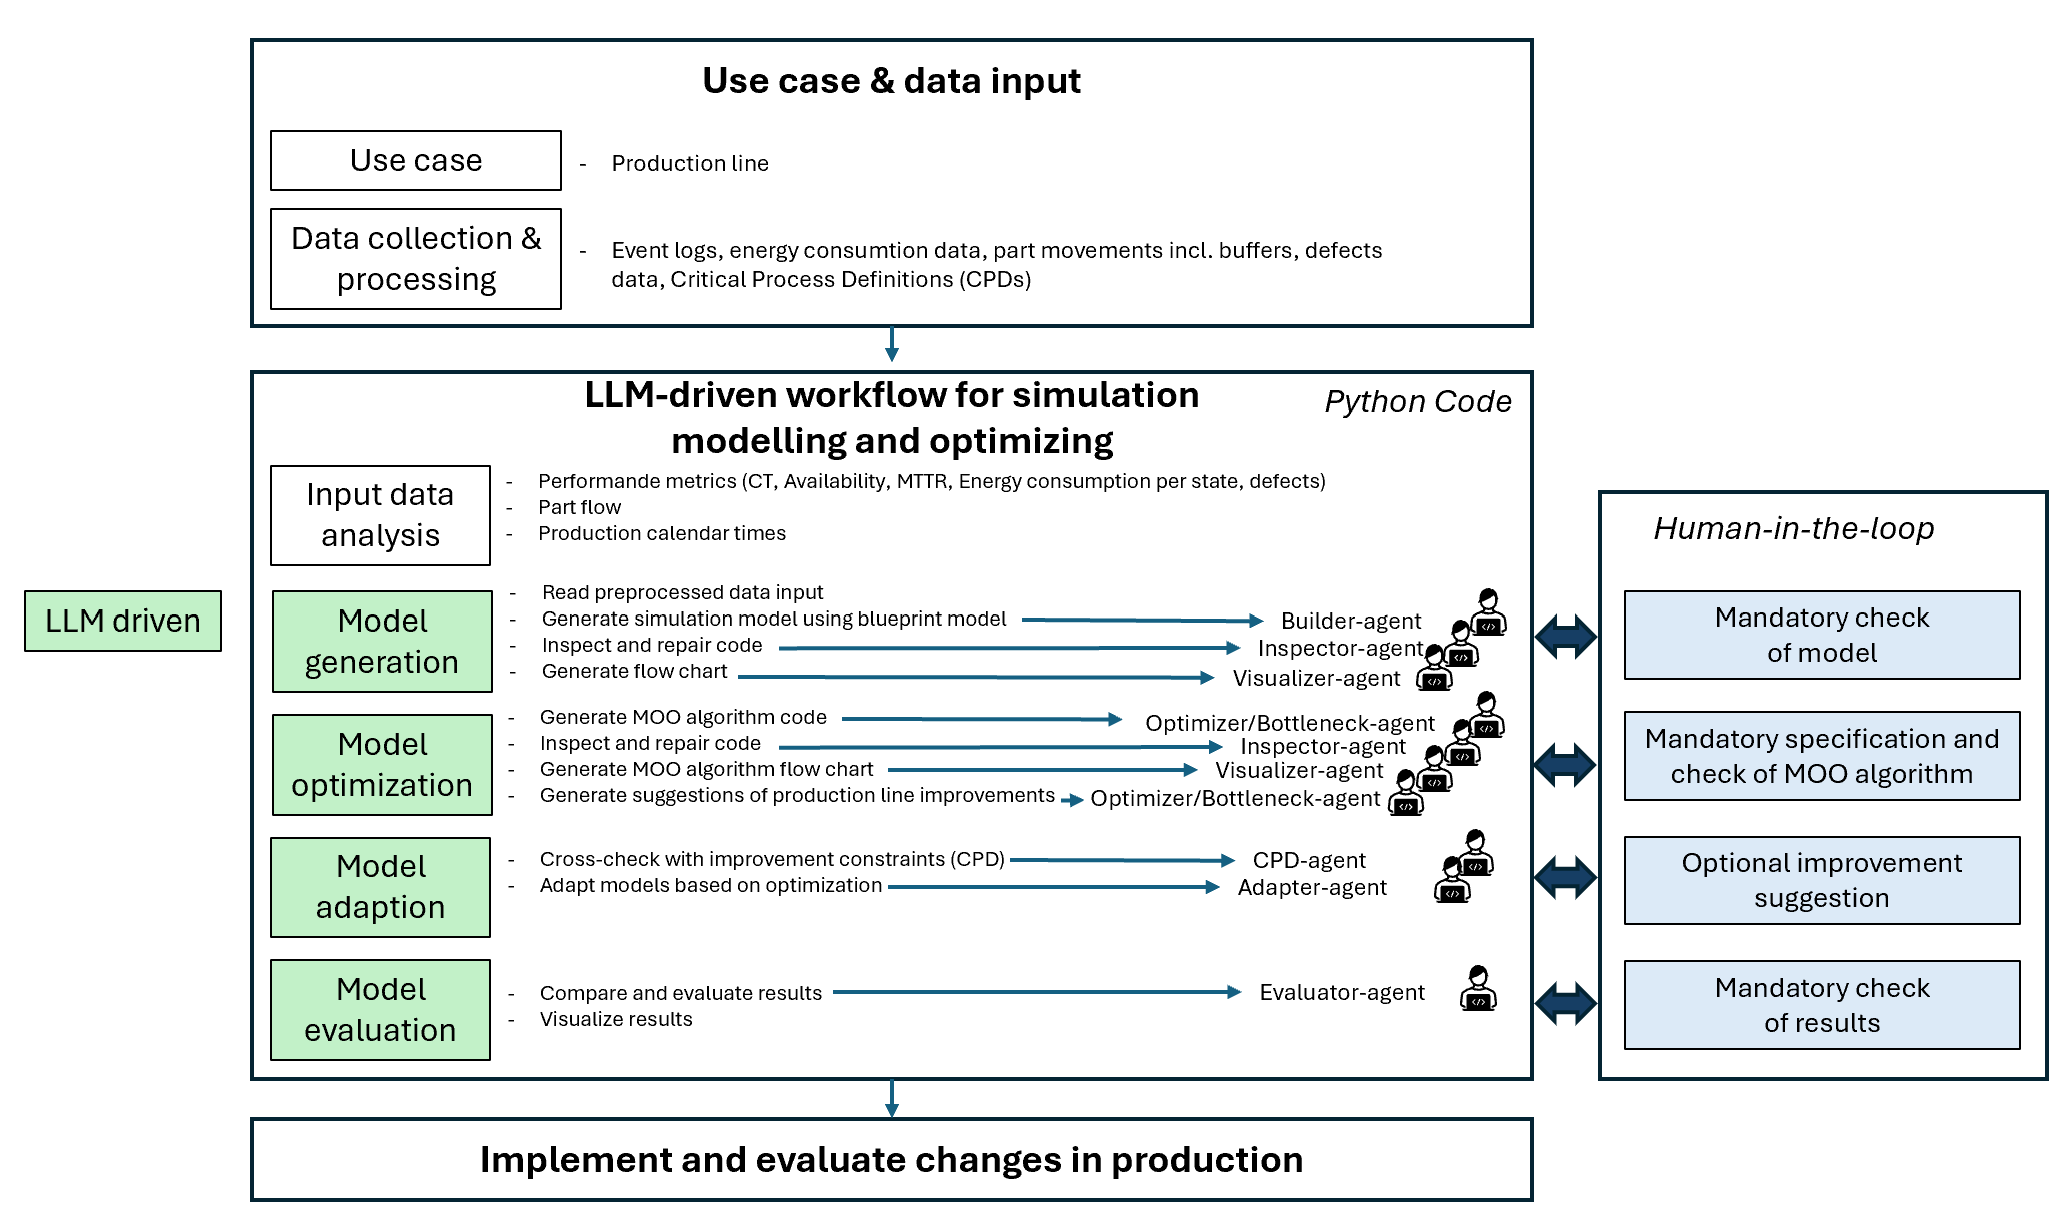
\includegraphics[width=0.9\textwidth]{figs/ModellingProcess.png}                                                         
  \caption{High-level view of the framework. The middle band groups the five pipeline stages -- data preparation, DES   
  generation, MOO, bottleneck analysis, and adaptation/evaluation -- and links each responsible LLM agent to a          
  human-in-the-loop touchpoint on the right.}                                                                           
  \label{fig:ModellingProcess}                                                                                          
  \end{figure}                                                                                                          
                                                                                                                        
  \begin{figure}[!htb]                                                                                                    
  \centering                                                                                                            
  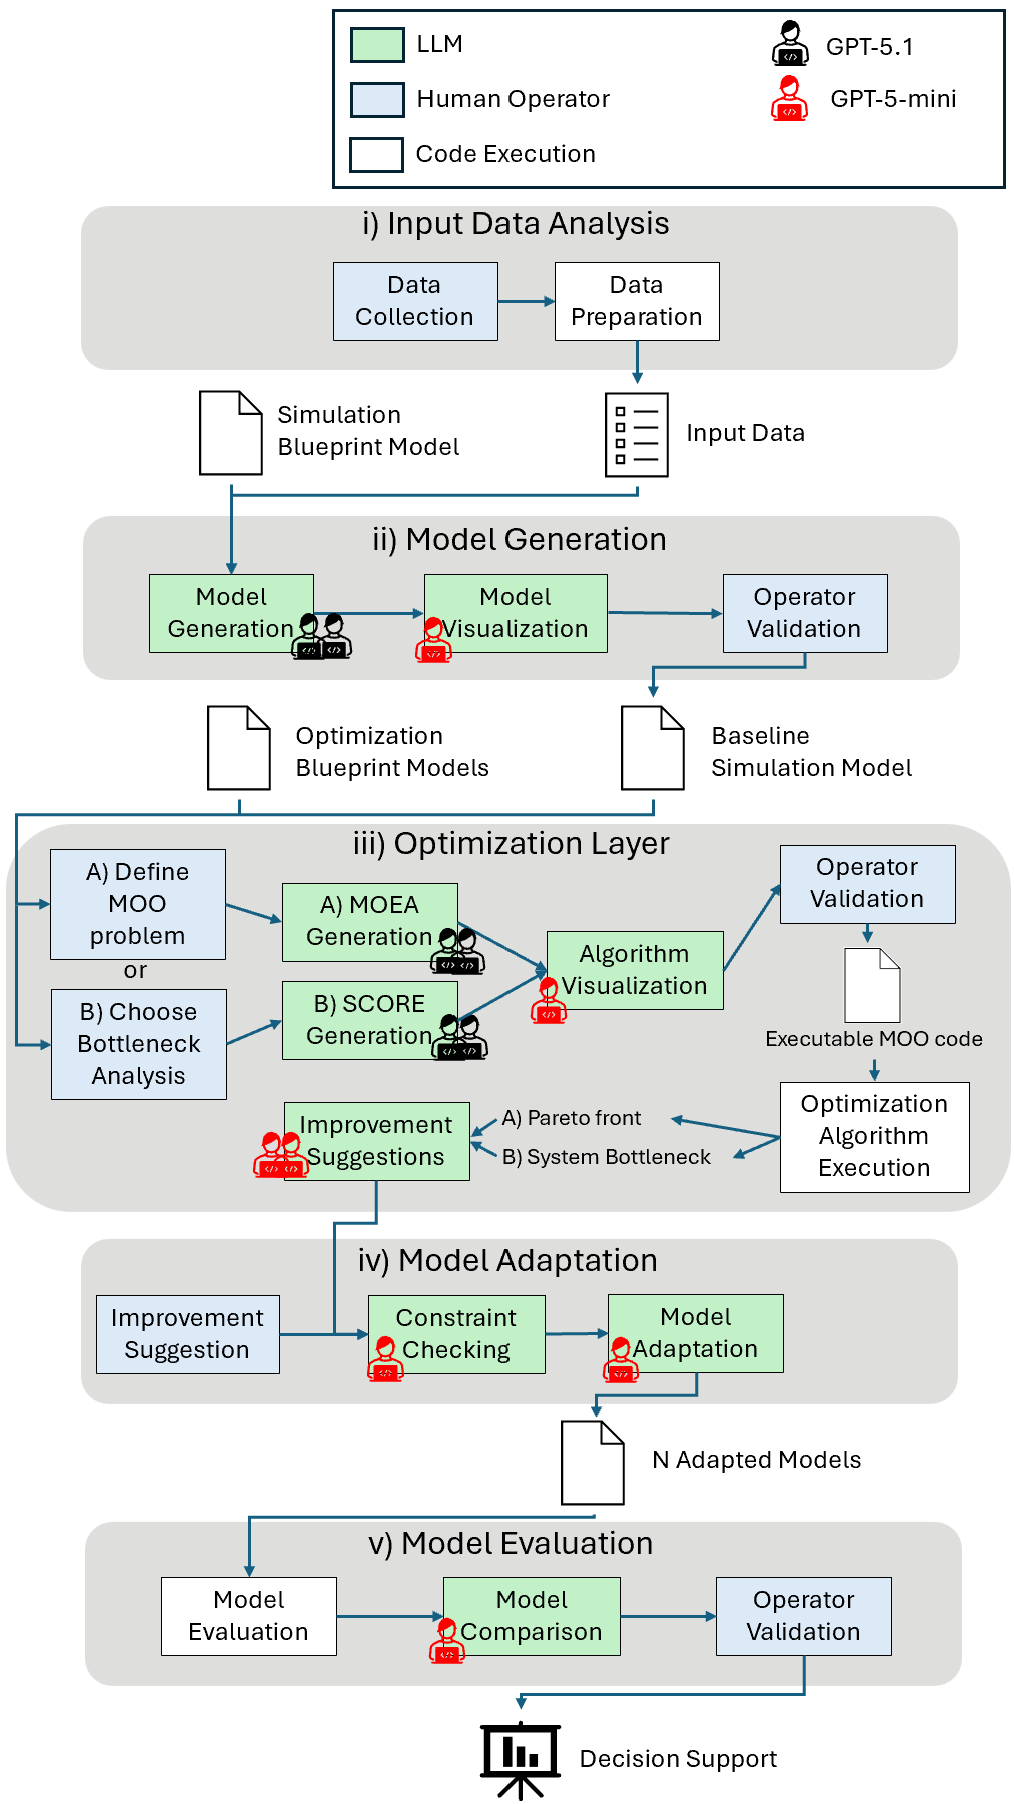
\includegraphics[width=0.7\textwidth]{figs/FrameworkOverview.png}                                                     
  \caption{Detailed pipeline view. Rounded blocks denote LLM-driven steps, shaded blocks denote human-operator steps,   
  and rectangular blocks denote deterministic code execution. Document icons mark the artifacts exchanged between stages
   (simulation and MOO blueprints, baseline DES, executable MOEA code, adapted DES variants, bottleneck report).        
  Stage~S3/S4 bifurcates into (A)~NSGA-II MOEA generation for multi-objective optimization or (B)~automated SCORE for   
  bottleneck analysis.}                                     
  \label{fig:FrameworkOverview}
  \end{figure}                                                                                                          
                                                                                                                        
  \begin{table}[!H]                                                                                                  
  \centering                                                                                                            
  \caption{Components of the framework, with type, primary responsibility, inputs, outputs, and pipeline stage.         
  LLM~=~large-language-model agent; Det.~=~deterministic Python module; HITL~=~human-in-the-loop checkpoint. LLM tier   
  used in the reported experiments: GPT-5.1 for code generation and adaptation; GPT-5-mini for visualization and
  evaluation.}                                                                                                          
  \label{tab:agents}                                        
  \resizebox{\textwidth}{!}{%                                                                                           
  \begin{tabular}{p{2.4cm} p{0.8cm} p{4.0cm} p{3.6cm} p{3.6cm} p{1.2cm}}                                                
  \toprule                                                                                                              
  \textbf{Component} & \textbf{Type} & \textbf{Responsibility} & \textbf{Input} & \textbf{Output} & \textbf{Stage} \\   
  \midrule                                                                                                              
  Log preprocessor & Det. & Extract per-machine cycle-time, MTBF, MTTR, energy profiles from the raw event log &        
  Production event log (CSV) & Structured line statistics (JSON) & S1 \\ \addlinespace                                  
  CPD module & Det. & Detect regime changes / periodic stops in the event log; produce production-calendar hints & Line 
  statistics & Calendar and stop-window annotations & S1 \\ \addlinespace                                               
  Builder agent & LLM & Generate the SimPy DES of the line from statistics and the simulation blueprint & Line
  statistics, simulation blueprint & Executable SimPy DES (Python) & S2 \\ \addlinespace                                
  Visualizer agent & LLM & Produce a Mermaid diagram of the generated DES for practitioner inspection & Executable DES &
   Mermaid diagram & S2 \\ \addlinespace                                                                                
  Optimizer agent & LLM & Generate a tailored NSGA-II MOEA that wraps the generated DES, using the MOO blueprint &
  Executable DES, MOO blueprint, objectives (via HITL) & Executable MOEA (Python), Pareto front (CSV) & S3 \\           
  \addlinespace                                             
  Bottleneck agent & LLM & Instantiate the automated SCORE formulation over the DES, run the optimization, report a     
  ranked alleviation list & Executable DES, SCORE blueprint & Ranked alleviation list with natural-language rationale & 
  S4 \\ \addlinespace
  Adapter agent & LLM & Modify the DES in response to a SCORE-derived instruction or a natural-language user request &  
  Executable DES, adaptation instruction & Adapted DES variant & S5 \\ \addlinespace                                    
  Evaluator agent & LLM & Produce KPI deltas across DES versions and their Pareto configurations & DES versions, KPI
  results & Comparative KPI report & S5 \\ \addlinespace                                                                
  Inspector agent & LLM & Repair syntactically or structurally broken generated code through error-driven prompting;
  bounded retry budget & Failing code, traceback & Patched code & S2--S5 (cross-cutting) \\ \addlinespace               
  HITL checkpoints & HITL & Elicit objectives, MOEA hyperparameters, Pareto-point preferences, and adaptation choices
  from the practitioner & Structured terminal prompts & User selections; defaults if omitted & S3, S4, S5 \\            
  \bottomrule                                               
  \end{tabular}                                                                                                         
  }                                                                                                                     
  \end{table}                                                                                                           
                                                                                                                        
  \subsection{Stage S1: Data preparation}\label{sec:framework-s1}                                                       
                                                            
  The framework consumes a raw production event log whose schema is a case identifier, a machine name, event start and  
  end timestamps, a machine state token, and an energy consumption per event. The log preprocessor is a deterministic
  Python module: it computes per-machine cycle-time distributions, MTBF and MTTR estimates, and per-state power         
  profiles, and packages them as a structured JSON summary that is passed to the builder agent. A companion
  deterministic change-point-detection (CPD) module scans the log for regime changes and for periodic stops (shifts,
  weekends, maintenance windows), and augments the summary with a production-calendar description. No LLM call is issued
   in this stage; the summary is fully reproducible from the log.

  \subsection{Stage S2: DES model generation}\label{sec:framework-s2}                                                   
   
  The builder agent receives the structured line statistics from stage S1 together with the \emph{simulation blueprint} 
  (Section~\ref{sec:framework-crosscut}), and emits an executable SimPy model of the line. The blueprint fixes the
  structural skeleton -- machines, buffers, splitters/mergers, the run-loop, and the KPI collection code -- while the   
  line statistics fill in numerical parameters. The visualizer agent, invoked in parallel, produces a Mermaid diagram of
   the generated DES so that a non-expert practitioner can inspect the topology before running any optimization. If the
  generated code fails to execute, control passes to the inspector agent (Section~\ref{sec:framework-crosscut}) which
  repairs the code before returning control to stage S3.

  \subsection{Stage S3: Multi-objective optimization}\label{sec:framework-s3}                                           
   
  The optimizer agent takes the executable DES, the MOO blueprint, and a set of user-selected objectives and decision   
  variables (chosen at an HITL checkpoint; defaults are provided for a fully unattended run), and emits a tailored
  NSGA-II MOEA that wraps the DES. The MOO blueprint fixes the search skeleton: problem definition, decision-variable   
  encoding, selection/crossover/mutation operators, and the termination criterion. Hyperparameters are proposed by the
  optimizer agent within literature-typical ranges and confirmed at a second HITL checkpoint. The MOEA is executed in
  Python; each candidate solution is evaluated by one simulation run of the generated DES, and the algorithm returns a
  Pareto front of non-dominated buffer configurations as a CSV artifact. A third HITL checkpoint lets the practitioner
  select a subset of Pareto points for further evaluation; in the fully unattended mode, the optimizer agent selects
  three canonical points itself (lowest-WIP, knee, highest-TH).

  \subsection{Stage S4: Automated bottleneck analysis}\label{sec:framework-s4}                                          
   
  Stage S4 instantiates the SCORE method \citep{Bernedixen2015} as an LLM-generated MOO over the executable DES. The    
  bottleneck agent reads the DES, identifies each machine and its parameters, and emits the SCORE problem definition:
  (i)~a discretized improvement variable per-machine attribute (availability, MTTR, PT) with a defined range and    
  step size, (ii)~two objectives -- maximize system throughput and minimize the total number of improvements applied --
  and (iii)~an NSGA-II search over the resulting improvement space. The agent then runs the optimization and reports a
  frequency analysis over the resulting non-dominated solutions, producing a ranked list of alleviation actions
  accompanied by short natural-language explanations. Ranges and step sizes are proposed by the bottleneck agent from
  the machine parameters and can be adjusted by the practitioner at an HITL checkpoint.

  \subsection{Stage S5: Model adaptation and evaluation}\label{sec:framework-s5}                                        
   
  The adapter agent modifies the DES in response to either a SCORE-derived instruction from stage S4 (for example,      
  ``reduce the process time of Presses cell 2 by 10\%'') or a natural-language instruction from the practitioner (for
  example, ``double the antecedent buffer of Presses cell 2''). Adaptation preserves the DES structure and modifies only
   the numerical parameters that the instruction targets, so that the adapted variant remains directly comparable to the
   baseline. The evaluator agent then re-runs the adapted DES, compares the resulting TH, WIP, and SEC to the baseline
  and to the FACTS reference, and produces a natural-language KPI report that highlights the direction and magnitude of
  each change. Both stages use the inspector agent for code-repair, but neither generates new structural code; the error types in Stage~S5 are therefore quantitatively different from those in stages~S2--S4 (cf.\ the syntax / structural / reasoning breakdown in Table~\ref{tab:ablation_errors}).
  
  %Both stages use the inspector agent for code-repair, but neither generates new structural code; the
  %failure modes faulty code are therefore quantitatively different from those of stages S2--S4.

  \subsection{Cross-cutting components: blueprints, inspector, HITL}\label{sec:framework-crosscut}                      
   
  \paragraph{Blueprints.} Three blueprints are used: the \emph{simulation blueprint} for stage S2, the \emph{MOO        
  blueprint} for stage S3, and the \emph{SCORE blueprint} for stage S4. Each blueprint is a short, executable Python
  skeleton that encodes the recurring structure of the target artifact. Concretely, the simulation blueprint contains:  
  (i)~a \texttt{DelayBuffer} class with capacity-limited enqueue/dequeue and in-transit accounting; (ii)~a
  \texttt{Machine} class with availability-driven breakdowns, process-time and power accounting, and a defect-rate hook;
   (iii)~splitter, merger, and forwarder utilities; (iv)~a \texttt{run\_simulation(seed)} entry point that instantiates
  the topology, applies the warm-up, samples the WIP process, and returns a KPI dictionary. The MOO blueprint contains:
  a \texttt{pymoo}-based problem class with decision-variable ranges and constraint hooks, an NSGA-II configuration with
   simulated binary crossover (SBX) and polynomial mutation (PM) operators, and a runner that persists the Pareto front to CSV. The SCORE blueprint contains: a
  \texttt{ScoreProblem} class that parameterizes each machine's improvement variables, the bi-objective formulation, and
   the post-hoc frequency-ranking routine. Each blueprint is under 300 lines and is distributed with the framework's
  source code (Section~\ref{sec:data-availability}).

  \paragraph{LLM prompts.} Each LLM agent is driven by a system prompt that fixes its role and output format, and a user
   prompt that supplies the stage-specific inputs. For the builder agent the system prompt establishes the SimPy target,
   the required entry point signature, and the requirement to reuse the classes defined in the simulation blueprint; the
   user prompt provides the JSON line statistics and cites the blueprint by name. For the optimizer agent the system
  prompt fixes the \texttt{pymoo} target, the encoding of decision variables, and the constraint model; the user prompt
  provides the target objectives, decision variables, and hyperparameter overrides. The bottleneck and adapter prompts
  follow the same pattern. All prompts request JSON- or code-only responses to enable deterministic parsing.

  \paragraph{Inspector agent.} Every stage that generates executable code executes it in a sandboxed subprocess. If the 
  code raises an exception, the inspector agent receives the traceback and the failing source, produces a targeted
  patch, and the framework re-attempts execution. Repair is bounded to four attempts per generation event to avoid      
  pathological loops. In the reported experiments (Section~\ref{sec:results-ablation}) the inspector successfully
  repairs the majority of transient generation failures without any user intervention.

  \paragraph{HITL checkpoints.} The framework exposes six HITL checkpoints across the pipeline: (H1)~confirmation of the parsed line topology and machine parameters after stage S1, (H2)~confirmation of the visualized DES structure after stage S2, (H3)~selection of MOO objectives and decision variables at the start of stage S3, (H4)~confirmation of MOEA  hyperparameters within stage S3, (H5)~selection of Pareto points to evaluate further at the end of stage S3, and (H6)~confirmation or overriding of SCORE improvement ranges within stage S4. All six checkpoints are presented as structured terminal prompts with defaults; when defaults are accepted throughout, the framework runs unattended. %The ablation in Section~\ref{sec:results-ablation} isolates the contribution of these checkpoints to the workflow.

                                                            
                                                                                                                        
  % ======================================================================
  % 4. Case study and evaluation methodology                                                                            
  % ======================================================================                                              
  \section{Case study and evaluation methodology}\label{sec:case}                                                       
                                                                                                                        
  \subsection{Production line (Case~A)}\label{sec:case-line}                                                            
                                                                                                                        
  The framework is evaluated on a real automotive production line at a large Swedish OEM, referred to as Case~A. The    
  line comprises seven operations connected by six intermediate buffers (Figure~\ref{fig:caseA}). Parts enter through a
  loading robot, pass a conveyor belt and a washing machine, and reach a Hantering (handling) cell that splits the flow 
  across two parallel press cells operating in parallel. The two press branches are re-merged into a shared post-press
  buffer, and the flow terminates in a quality-station cell. Each operation is characterized by a cycle time, an
  availability, a mean time to repair, a working-power draw, and an idle-power draw; the quality-station additionally
  has a defect rate. The full parameter set is provided in the released repository
  (Section~\ref{sec:data-availability}); representative values are given in Table~\ref{tab:machine_params}.

  \begin{figure}[]                                                                                                 
  \centering
  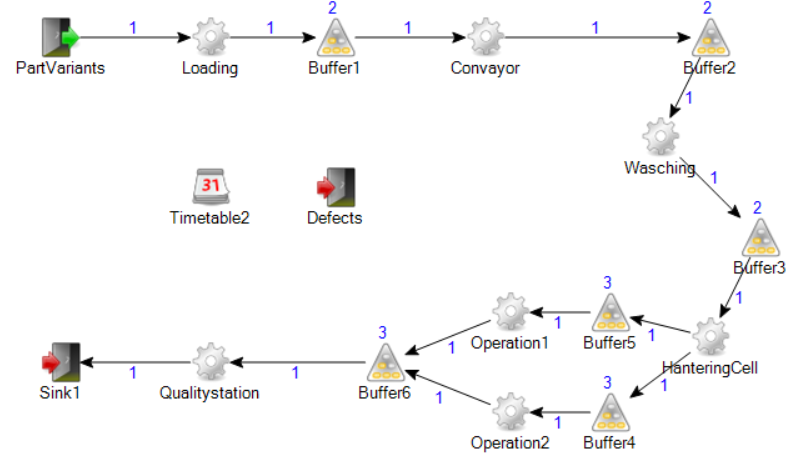
\includegraphics[width=0.5\textwidth]{figs/CaseA_facts_line.png}                                                      
  \caption{Case~A production-line layout used for the experiments. Six intermediate buffers (Buf~1--6) separate the     
  seven operations. Two press cells operate in parallel on the branched flow between Buf~4/5 and Buf~6.}                
  \label{fig:caseA}                                                                                                     
  \end{figure}                                                                                                          
                                                                                                                        
  \begin{table}[ ]                                                                                                  
  \centering                                                                                                            
  \caption{Case~A machine parameters used in the DES. Cycle time in seconds; availability in percent; MTTR in seconds;  
  working and idle power in kW. The quality-station cell additionally has a defect rate of $0.089$.}                    
  \label{tab:machine_params}                                                                                            
  \begin{tabular}{@{}l r r r r r@{}}                                                                                    
  \toprule                                                                                                              
  \textbf{Machine} & \textbf{Cycle time (s)} & \textbf{Avail.\ (\%)} & \textbf{MTTR (s)} & \textbf{Work. pow.\ (kW)} &  
  \textbf{Idle pow.\ (kW)} \\                                                                                           
  \midrule                                                                                                              
  Loading robot        & 12   & 90.49 & 68  & 0.72  & 0.25 \\                                                           
  Conveyor belt        & 6    & 100   & --  & 0.00  & 0.00 \\                                                           
  Washing machine      & 14   & 80.89 & 269 & 35.24 & 4.28 \\                                                           
  Hantering cell       & 25   & 97.79 & 74  & 0.74  & 0.50 \\                                                           
  Presses cell 1       & 175  & 87.79 & 73  & 1.28  & 1.25 \\                                                           
  Presses cell 2       & 176  & 87.69 & 74  & 1.27  & 1.25 \\                                                           
  Quality station cell & 41   & 85.87 & 66  & 0.84  & 0.58 \\                                                           
  \bottomrule                                                                                                           
  \end{tabular}                                                                                                         
  \end{table}                                                                                                           
                                                                                                                        
  The input event log covers several weeks of production and provides, for each event, a case identifier, a machine     
  name, event start and end timestamps, a machine state token (working, idle, blocked, failed), and an energy
  consumption per event. Weekly production windows are Monday--Friday 07:00--17:00 and Saturday 07:00--12:00; the CPD   
  module extracts these windows automatically from the log. 

  \subsection{Optimization problem}\label{sec:case-problem}                                                             
   
The decision variables are the capacities of the six intermediate buffers, each an integer in the range $[1, 10]$. The MOO scenario evaluated here (Scenario~S1) maximizes TH and minimizes WIP, subject to the constraint that the  
  total buffer capacity does not exceed~50 parts. A second scenario, minimizing WIP and SEC, was designed but not   
  run as a standalone MOEA because the systematic SEC over-estimate documented in Section~\ref{sec:results-fidelity}
  would render its hypervolume comparison uninformative; a full SEC-oriented evaluation is deferred to future work  
  (Section~\ref{sec:conclusion}). 
  SEC in    
  this study is the ratio of total machine energy consumption (working plus idle) to total produced parts, in kWh per
  part, and TH is measured in produced parts per hour after warm-up.

  \subsection{NSGA-II configuration and simulation setup}\label{sec:case-facts}                                         
   
  The MOEA is NSGA-II with SBX and PM genetic operators. Table~\ref{tbl:hyper} lists   
  the hyperparameters. A population of 50 candidates is evolved over 10 generations with 3 simulation replications per
  candidate; this gives a simulation budget of $50 \times 10 \times 3 = 1{,}500$ DES runs per optimization scenario. The
   population size and generation count match the default configuration of the FACTS Analyzer reference on the same
  problem, which ensures fairness in the head-to-head comparison. SBX with $p = 0.9$ and $\eta = 15$, and PM with $p =
  1/6$ and $\eta = 20$, are standard defaults in the NSGA-II literature \citep{Deb2002nsga2}. The initial population is
  generated by integer uniform sampling of each buffer capacity within its permitted range. The simulated horizon of
  $691{,}200$~s (eight days) with a warm-up of $86{,}400$~s (one day) matches the default configuration of FACTS
  Analyzer for the same line; a formal Welch-style steady-state analysis is left as an item of future work
  (Section~\ref{sec:discussion-limits}).

  \begin{table}[ ]                                                                                                  
  \caption{NSGA-II hyperparameters used in the case study. Population size and generations match the FACTS Analyzer
  reference configuration.}                                                                                             
  \label{tbl:hyper}                                         
  \centering                                                                                                            
  \begin{tabular}{@{}l l@{}}                                                                                            
  \toprule                                                                                                              
  \textbf{Parameter} & \textbf{Value} \\                                                                                
  \midrule                                                                                                              
  Algorithm & NSGA-II \citep{Deb2002nsga2} \\                                                                           
  Population size & 50 \\                                                                                               
  Generations & 10 \\                                                                                                   
  Simulation replications per candidate & 3 \\                                                                          
  Initial population & integer uniform sampling on $[1, 10]$ per buffer \\                                              
  Crossover operator & SBX, $p = 0.9$, $\eta = 15$ \\                                                                   
  Mutation operator & PM, $p = 1/6$, $\eta = 20$ \\                                                                     
  Simulated horizon & $691{,}200$~s (8 days) \\                                                                         
  Warm-up period & $86{,}400$~s (1 day) \\                                                                              
  Constraint & total buffer capacity $\leq 50$ \\                                                                       
  \bottomrule                                                                                                           
  \end{tabular}                                                                                                         
  \end{table}                                                                                                           
                                                                                                                        
  \subsection{Reference implementation (FACTS Analyzer)}\label{sec:case-ref}                                            
                                                                                                                        
  The same production line, event log, and optimization problem are implemented independently in FACTS Analyzer using   
  the same NSGA-II configuration (with the exception of the operator $\eta$ values, which are not user-accessible in the
   tool). The FACTS implementation is used as the reference against which generation fidelity, solution quality, and    
  bottleneck rankings are compared.                         

  \subsection{Evaluation methodology}\label{sec:case-evaluation}                                                        
   
  Four evaluation dimensions are defined \emph{a priori} and reported in Section~\ref{sec:results}: (i)~\emph{fidelity},
   (ii)~\emph{solution quality}, (iii)~\emph{performance retention under sustained perturbation}, and (iv)~\emph{operational cost}.
                                                                                                                        
  \emph{Fidelity} is the absolute deviation of TH, WIP, and SEC produced by the framework-generated DES from the FACTS  
  reference under identical model parameters. It is reported both for the initial (unoptimized) model and for three
  adapted variants corresponding to the three Pareto points selected in Section~\ref{sec:results-moo}. Standard         
  deviations across the ten baseline seeds are reported alongside means so that the reader can assess run-to-run
  variability.

  \emph{Solution quality} is the hypervolume (HV) of the Pareto front returned by each optimizer, computed against a    
  common nadir point derived from the worst KPI values observed across all feasible MOO solutions and further worsened
  by ten percent to guarantee dominance. Concretely, the nadir used for Scenario~S1 is $(\mathrm{WIP} = 59.4,           
  \mathrm{TH} = 22.6)$. HV is reported as mean and standard deviation over the baseline seeds for which the LLM pipeline returned a feasible MOO artifact (nine of ten seeds for the Baseline configuration; see Section~\ref{sec:results-fidelity}), and a Wilcoxon rank-sum test
  on the per-seed HV values is used to test whether the framework's HV differs significantly from the FACTS reference's
  HV. Bottleneck-ranking quality is reported as the agreement between the framework's SCORE ranking and the FACTS SCORE
  ranking on the top-$k$ alleviation actions, with $k \in \{3, 4, 5\}$.

  \emph{Performance retention under sustained perturbation} is the fraction of nominal TH retained when the DES is stress-tested under three sustained parameter-perturbation scenarios ($D_1$, $D_2$, $D_3$; see Section~\ref{sec:resilience}). For a Pareto configuration $x$ and perturbation scenario $d$, retention is $R_d(x) = TH_d(x) / TH_\mathrm{nom}(x)$, and the worst-case performance-retention score is $R_\mathrm{worst}(x) = \min_d R_d(x)$, following the retention-of-performance perspective reviewed by \citet{Hosseini2016}. This metric captures one operational dimension of resilience, namely the ability to maintain production performance under degraded operating conditions; it does not capture post-disruption recovery dynamics, recovery time, or adaptation trajectories.          

  \emph{Operational cost} is reported as the number of OpenAI API calls, the number of input and output tokens, the     
  resulting USD cost per completed study, and the end-to-end wall-clock time. Reporting all four allows the reader to
  project the cost of scaling to a different LLM tier or to a longer optimization budget.                               
                                                            
                                                                                         
  % ======================================================================
  % 5. Results                                                                                                          
  % ======================================================================                                              
  \section{Results}\label{sec:results}                                                                                  
                                                                                                                        
  Results are reported along the four evaluation dimensions defined in Section~\ref{sec:case-evaluation}: fidelity      
  (\S~\ref{sec:results-fidelity}), solution quality (\S~\ref{sec:results-moo} and \S~\ref{sec:results-bn}), a component 
  ablation (\S~\ref{sec:results-ablation}), and operational cost (\S~\ref{sec:results-cost}). The performance-retention dimension is reported separately in Section~\ref{sec:resilience}.   

  

  \subsection{Fidelity}\label{sec:results-fidelity}   

For the baseline configuration, the framework's DES of Case~A reproduces the KPIs of the FACTS Analyzer reference on the initial (unoptimized) model and on three adapted variants corresponding to the three Pareto points selected in Section~\ref{sec:results-moo} (Table~\ref{tab:facts_python_comparison}). TH agreement is within 1~\% across all four versions. WIP agreement is within 3~\% on the unoptimized model and on the lowest-WIP configuration (V1), and grows to approximately 9~\% at the knee-point (V2) and highest-TH (V3) configurations. This configuration-dependent WIP discrepancy is documented here and discussed further in Section~\ref{sec:discussion-validity}; its mechanistic origin has not been fully characterized in the current work.
%, a discrepancy analyzed in Section~\ref{sec:discussion-validity}. 
SEC is systematically higher in the framework-generated model by approximately 3~\% across all four versions, an accounting difference in how transition intervals are classified between the SimPy blueprint and FACTS Analyzer. The SEC discrepancy would affect any SEC-oriented MOO scenario (a full evaluation of which is deferred to future work) but does not   
  affect the TH/WIP scenario (S1) or the bottleneck ranking.

The values in Table~\ref{tab:facts_python_comparison} are means over ten random seeds $\{11, 22, 33, 44, 55, 66, 77, 88, 99, 110\}$ using the
released canonical Python DES. On the unoptimized model, the framework's TH averages $27.15 \pm 0.17$~parts/h against the reference value of $27.31$~parts/h ($-0.60$~\% deviation), and its WIP averages $18.16 \pm 0.13$~parts against the reference value of $18.43$~parts ($-1.46$~\% deviation). One of the ten seeds (seed~88) additionally exhibits a known LLM code-generation failure in the per-seed model-build reported in Section~\ref{sec:results-cost}; that failure affects  Table~\ref{tab:seed_metrics} but not Table~\ref{tab:facts_python_comparison}, and the affected seed is excluded from the hypervolume computation described below following the convention adopted in the released dataset.






\begin{table}[ ]                                                               
  \centering                             
  \caption{Fidelity of the framework-generated DES against the FACTS Analyzer       
  reference. Framework values are ten-seed means ($\pm$ population standard         
  deviation) obtained by running the canonical released Python DES                  
  (\texttt{paper/resilience/des\_perturbable.py}) on seeds                          
  $\{11, 22, 33, 44, 55, 66, 77, 88, 99, 110\}$. FACTS values are the               
  corresponding FACTS Analyzer simulations of the same buffer configurations.       
  The three variants V1--V3 correspond to the three Pareto points selected in       
  Section~\ref{sec:results-moo}: V1~=~lowest-WIP, V2~=~knee-point,                  
  V3~=~highest-TH.}                        
  \label{tab:facts_python_comparison}                                               
  \begin{tabular}{@{}l l c c r r@{}}                                                
  \toprule                                                                          
  \textbf{Model} & \textbf{KPI} & \textbf{FACTS} & \textbf{Framework} &             
  \textbf{Abs.\ diff.} & \textbf{\% diff.} \\                                       
  \midrule                                                  
  \textbf{Initial} & TH (parts/h)   & 27.31  & $27.15 \pm 0.17$    & 0.16   &       
  $-0.60$\% \\                                                                      
                   & WIP (parts)    & 18.43  & $18.16 \pm 0.13$    & 0.27   &
  $-1.46$\% \\                                                                      
                   & SEC (kWh/part) & 0.4373 & $0.4520 \pm 0.0019$ & 0.0148 &
  $+3.38$\% \\                                                                      
  \midrule                                                  
  \textbf{V1}      & TH (parts/h)   & 25.99  & $26.14 \pm 0.21$    & 0.15   &       
  $+0.58$\% \\                                                                      
                   & WIP (parts)    & 11.44  & $11.14 \pm 0.10$    & 0.30   &
  $-2.62$\% \\                                                                      
                   & SEC (kWh/part) & 0.4525 & $0.4650 \pm 0.0028$ & 0.0126 &
  $+2.78$\% \\                                                                      
  \midrule                                                  
  \textbf{V2}      & TH (parts/h)   & 27.12  & $27.08 \pm 0.15$    & 0.04   &       
  $-0.16$\% \\                                                                      
                   & WIP (parts)    & 15.47  & $14.13 \pm 0.39$    & 1.34   &
  $-8.66$\% \\                                                                      
                   & SEC (kWh/part) & 0.4392 & $0.4531 \pm 0.0028$ & 0.0139 &
  $+3.16$\% \\                                                                      
  \midrule                                                  
  \textbf{V3}      & TH (parts/h)   & 27.06  & $27.25 \pm 0.25$    & 0.19   &       
  $+0.69$\% \\                                                                      
                   & WIP (parts)    & 19.29  & $20.97 \pm 0.16$    & 1.68   &
  $+8.69$\% \\                                                                      
                   & SEC (kWh/part) & 0.4405 & $0.4510 \pm 0.0032$ & 0.0105 &
  $+2.39$\% \\                                                                      
  \bottomrule                                               
  \end{tabular}                                                                     
  \end{table}          





















  
   
  %For the baseline configuration, the framework generates a DES of Case~A whose KPIs closely match those of the FACTS Analyzer reference on the initial (unoptimized) model and on three adapted variants in which buffer capacities are modified according to LLM-selected points on the Pareto front (Table~\ref{tab:facts_python_comparison}). Differences   in TH and WIP remain within a few percent across all four versions; SEC is systematically higher in theframework-generated model by approximately 4~\%, an issue that is analyzed in Section~\ref{sec:discussion-validity} and traced to a well-understood accounting difference in how transition intervals are classified. The SEC discrepancyaffects the WIP/SEC scenario (S2) but not the TH/WIP scenario (S1) or the bottleneck ranking.

  %\begin{table}[ ]                                                                                                  
%  \centering
%  \caption{Fidelity of the framework-generated DES against the FACTS Analyzer reference. Values are single-run means for
%   a representative seed. The three variants V1--V3 correspond to the three Pareto points selected in                   
%  Section~\ref{sec:results-moo}: V1~=~lowest-WIP, V2~=~knee-point, V3~=~highest-TH.}
%  \label{tab:facts_python_comparison}                                                                                   
%  \begin{tabular}{@{}l l c c r r@{}}                                                                                    
%  \toprule                                                                                                              
%  \textbf{Model} & \textbf{KPI} & \textbf{FACTS} & \textbf{Framework} & \textbf{Abs.\ diff.} & \textbf{\% diff.} \\     
%  \midrule                                                                                                              
%  \textbf{Initial} & TH (parts/h) & 27.31 & 27.26 & 0.05 & $-0.18$\% \\                                                 
%                   & WIP (parts)  & 18.43 & 18.22 & 0.21 & $-1.14$\% \\                                                 
%                   & SEC (kWh/part) & 0.4373 & 0.4551 & 0.0178 & $+4.07$\% \\                                           
%  \midrule                                                                                                              
%  \textbf{V1}      & TH (parts/h) & 25.99 & 26.18 & 0.19 & $+0.73$\% \\                                                 
%                   & WIP (parts)  & 11.44 & 11.02 & 0.42 & $-3.67$\% \\                                                 
%                   & SEC (kWh/part) & 0.4524 & 0.4636 & 0.0112 & %$+2.48$\% \\                                           
%  \midrule                                                                                                              
%  \textbf{V2}      & TH (parts/h) & 26.59 & 26.14 & 0.45 & $-1.69$\% \\                                                 
%                   & WIP (parts)  & 11.53 & 11.22 & 0.31 & $-2.69$\% \\                                                 
%                   & SEC (kWh/part) & 0.4452 & 0.4643 & 0.0191 & $+4.29$\% \\                                           
%  \midrule                                                                                                              
%  \textbf{V3}      & TH (parts/h) & 26.76 & 26.19 & 0.57 & $-2.13$\% \\                                                 
%                   & WIP (parts)  & 11.37 & 11.27 & 0.10 & $-0.88$\% \\                                                 
%5                   & SEC (kWh/part) & 0.4432 & 0.4638 & 0.0206 & %$+4.65$\% \\                                           
%  \bottomrule                                                                                                           
%  \end{tabular}                                                                                                         
%  \end{table}        




                                                                                                                        
  %Across the ten baseline seeds reported in Section~\ref{sec:results-cost}, the framework's TH averages $27.30 \pm       0.06$~parts/h against the reference value of $27.31$~parts/h ($-0.05$~\% deviation), and its WIP averages $18.16 \pm  0.08$~parts against the reference value of $18.43$~parts ($-1.46$~\% deviation). One of the ten baseline seeds        (seed~88) exhibited a known model-build failure that produced degenerate KPIs; this seed is retained in the cost tablefor transparency but excluded from the fidelity means and from the hypervolume computation described below, followingthe convention adopted in the released dataset.








  

  \subsection{Solution quality: Pareto front and hypervolume}\label{sec:results-moo}                  

             
For Scenario~S1 (TH/WIP), the framework returns a Pareto front with 19                                            
  non-dominated solutions, corresponding to 15 unique buffer configurations                                         
  (Table~\ref{tab:paretofront}). Three points were selected from the front                                          
  in response to a ``best balance between WIP and throughput'' user prompt                                          
  at the HITL checkpoint~H5: the lowest-WIP corner (V1), a knee-point (V2),                                         
  and the highest-TH corner (V3). Their buffer configurations, together                                             
  with the ten-seed mean WIP and TH obtained by re-simulating each                                                  
  configuration with the canonical Python DES, are reported in                                                      
  Table~\ref{tab:suggestions}; the same three configurations are used as                                            
  V1, V2, and V3 throughout Sections~\ref{sec:results-fidelity}                                                     
  and~\ref{sec:resilience}. 

  Figure~\ref{fig:MOEAdata} superimposes the framework's Pareto front on the FACTS Analyzer reference front for the same scenario; the coordinates of the three selected points V1--V3 are listed in Table~\ref{tab:suggestions}.
                                                                                                                    
  The hypervolume of the framework's front, computed against the nadir                                              
  $(\mathrm{WIP}=59.4, \mathrm{TH}=22.6)$ defined in        
  Section~\ref{sec:case-evaluation}, is $235.53 \pm 1.63$ across nine                                               
  baseline seeds (excluding seed~88, cf.\ Section~\ref{sec:results-fidelity})                                       
  against $233.98 \pm 1.00$ for the FACTS reference on the same nadir over                                          
  ten seeds, a $+0.66$~\% mean improvement. A Wilcoxon rank-sum test on the                                         
  per-seed HV values gives $p = 0.05$: the null hypothesis of equal HV                                              
  distributions is not rejected at the conventional level, so the                                                   
  framework's front is comparable the FACTS                                               
  reference on Scenario~S1.                                                                                         
                                                                                                                    
  \begin{table}[ ]                                                                                               
  \centering                                                                                                        
  \caption{Pareto front returned by the framework for Scenario~S1 (TH/WIP)                                          
  on Case~A over one representative seed. All 19 rows are non-dominated on                                          
  (WIP, TH); the front collapses to 15 unique buffer configurations. Buf~1                                          
  through Buf~6 are, respectively, the PostLoading, PostConveyor,                                                   
  PostWashing, PrePress1, PrePress2, and PostPress1--2 buffer capacities.}                                          
  \label{tab:paretofront}                                                                                           
  \csvreader[                                                                                                       
      column names={                                                                                                
          generation_index = \genIdx,                                                                               
          individual_index = \indIdx,                                                                               
          PostLoadingBuffer_capacity = \capA,                                                                       
          PostConveyorBuffer_capacity = \capB,                                                                      
          PostWashingBuffer_capacity = \capC,                                                                       
          PrePress1Buffer_capacity = \capD,                                                                         
          PrePress2Buffer_capacity = \capE,                                                                         
          PostPress1_2_Buffer_capacity = \capF,                                                                     
          total_buffer_capacity = \capTotal,                                                                        
          wip = \valWip,                                                                                            
          throughput = \valTp                                                                                       
      },                                                                                                            
      tabular={c c | c c c c c c | c | c r},                                                                        
      table head=\toprule                                                                                           
          \textbf{Gen.} & \textbf{Ind.} & \textbf{Buf 1} & \textbf{Buf 2} &                                         
          \textbf{Buf 3} & \textbf{Buf 4} & \textbf{Buf 5} & \textbf{Buf 6}                                         
          & \textbf{Total} & \textbf{WIP} & \textbf{TH} \\ \midrule,                                                
      late after line=\\,                                                                                           
      table foot=\bottomrule                                                                                        
  ]{figs/moo_pareto_solutions.csv}{}{%                                                                              
      \genIdx & \indIdx & \capA & \capB & \capC & \capD & \capE & \capF                                             
      & \capTotal                                                                                                   
      & \num[round-mode=places, round-precision=2]{\valWip}                                                         
      & \num[round-mode=places, round-precision=2]{\valTp}                                                          
  }                                                                                                                 
  \end{table}                                                                                                       
                                                                                                                    
  \begin{table}[]                                                                                               
  \centering
  \caption{Three Pareto points selected at HITL checkpoint~H5 for further                                           
  evaluation (V1~=~lowest-WIP, V2~=~knee-point, V3~=~highest-TH). WIP and                                           
  TH are ten-seed means ($\pm$ population standard deviation) obtained by                                           
  re-simulating each buffer configuration with the canonical Python DES,                                            
  matching the Framework columns of                                                                                 
  Table~\ref{tab:facts_python_comparison}. Buf~1--6 are, respectively, the                                          
  PostLoading, PostConveyor, PostWashing, PrePress1, PrePress2, and                                                 
  PostPress1--2 buffer capacities.}                                                        
  \label{tab:suggestions}                                                                                           
  \begin{tabular}{@{}l c c c c c c c c r@{}}                                                                        
  \toprule                                                                                                          
  \textbf{Point} & \textbf{Buf 1} & \textbf{Buf 2} & \textbf{Buf 3} &                                               
  \textbf{Buf 4} & \textbf{Buf 5} & \textbf{Buf 6} & \textbf{Total} &                                               
  \textbf{WIP} & \textbf{TH} \\                                                                                     
  \midrule                                                                                                          
  V1 (lowest-WIP)  & 1 & 1 & 1 & 1 & 1 & 1 & 6  & $11.14 \pm 0.10$ & $26.14 \pm 0.21$ \\                            
  V2 (knee-point)  & 1 & 1 & 1 & 3 & 2 & 3 & 11 & $14.13 \pm 0.39$ & $27.08 \pm 0.15$ \\                            
  V3 (highest-TH)  & 1 & 3 & 4 & 3 & 4 & 2 & 17 & $20.97 \pm 0.16$ & $27.25 \pm 0.25$ \\                            
  \bottomrule                                                                                                       
  \end{tabular}                                                                                                     
  \end{table}                                                                                                       
                                                                                                                    
  \begin{figure}[ ]                                                                                              
  \centering                                                
  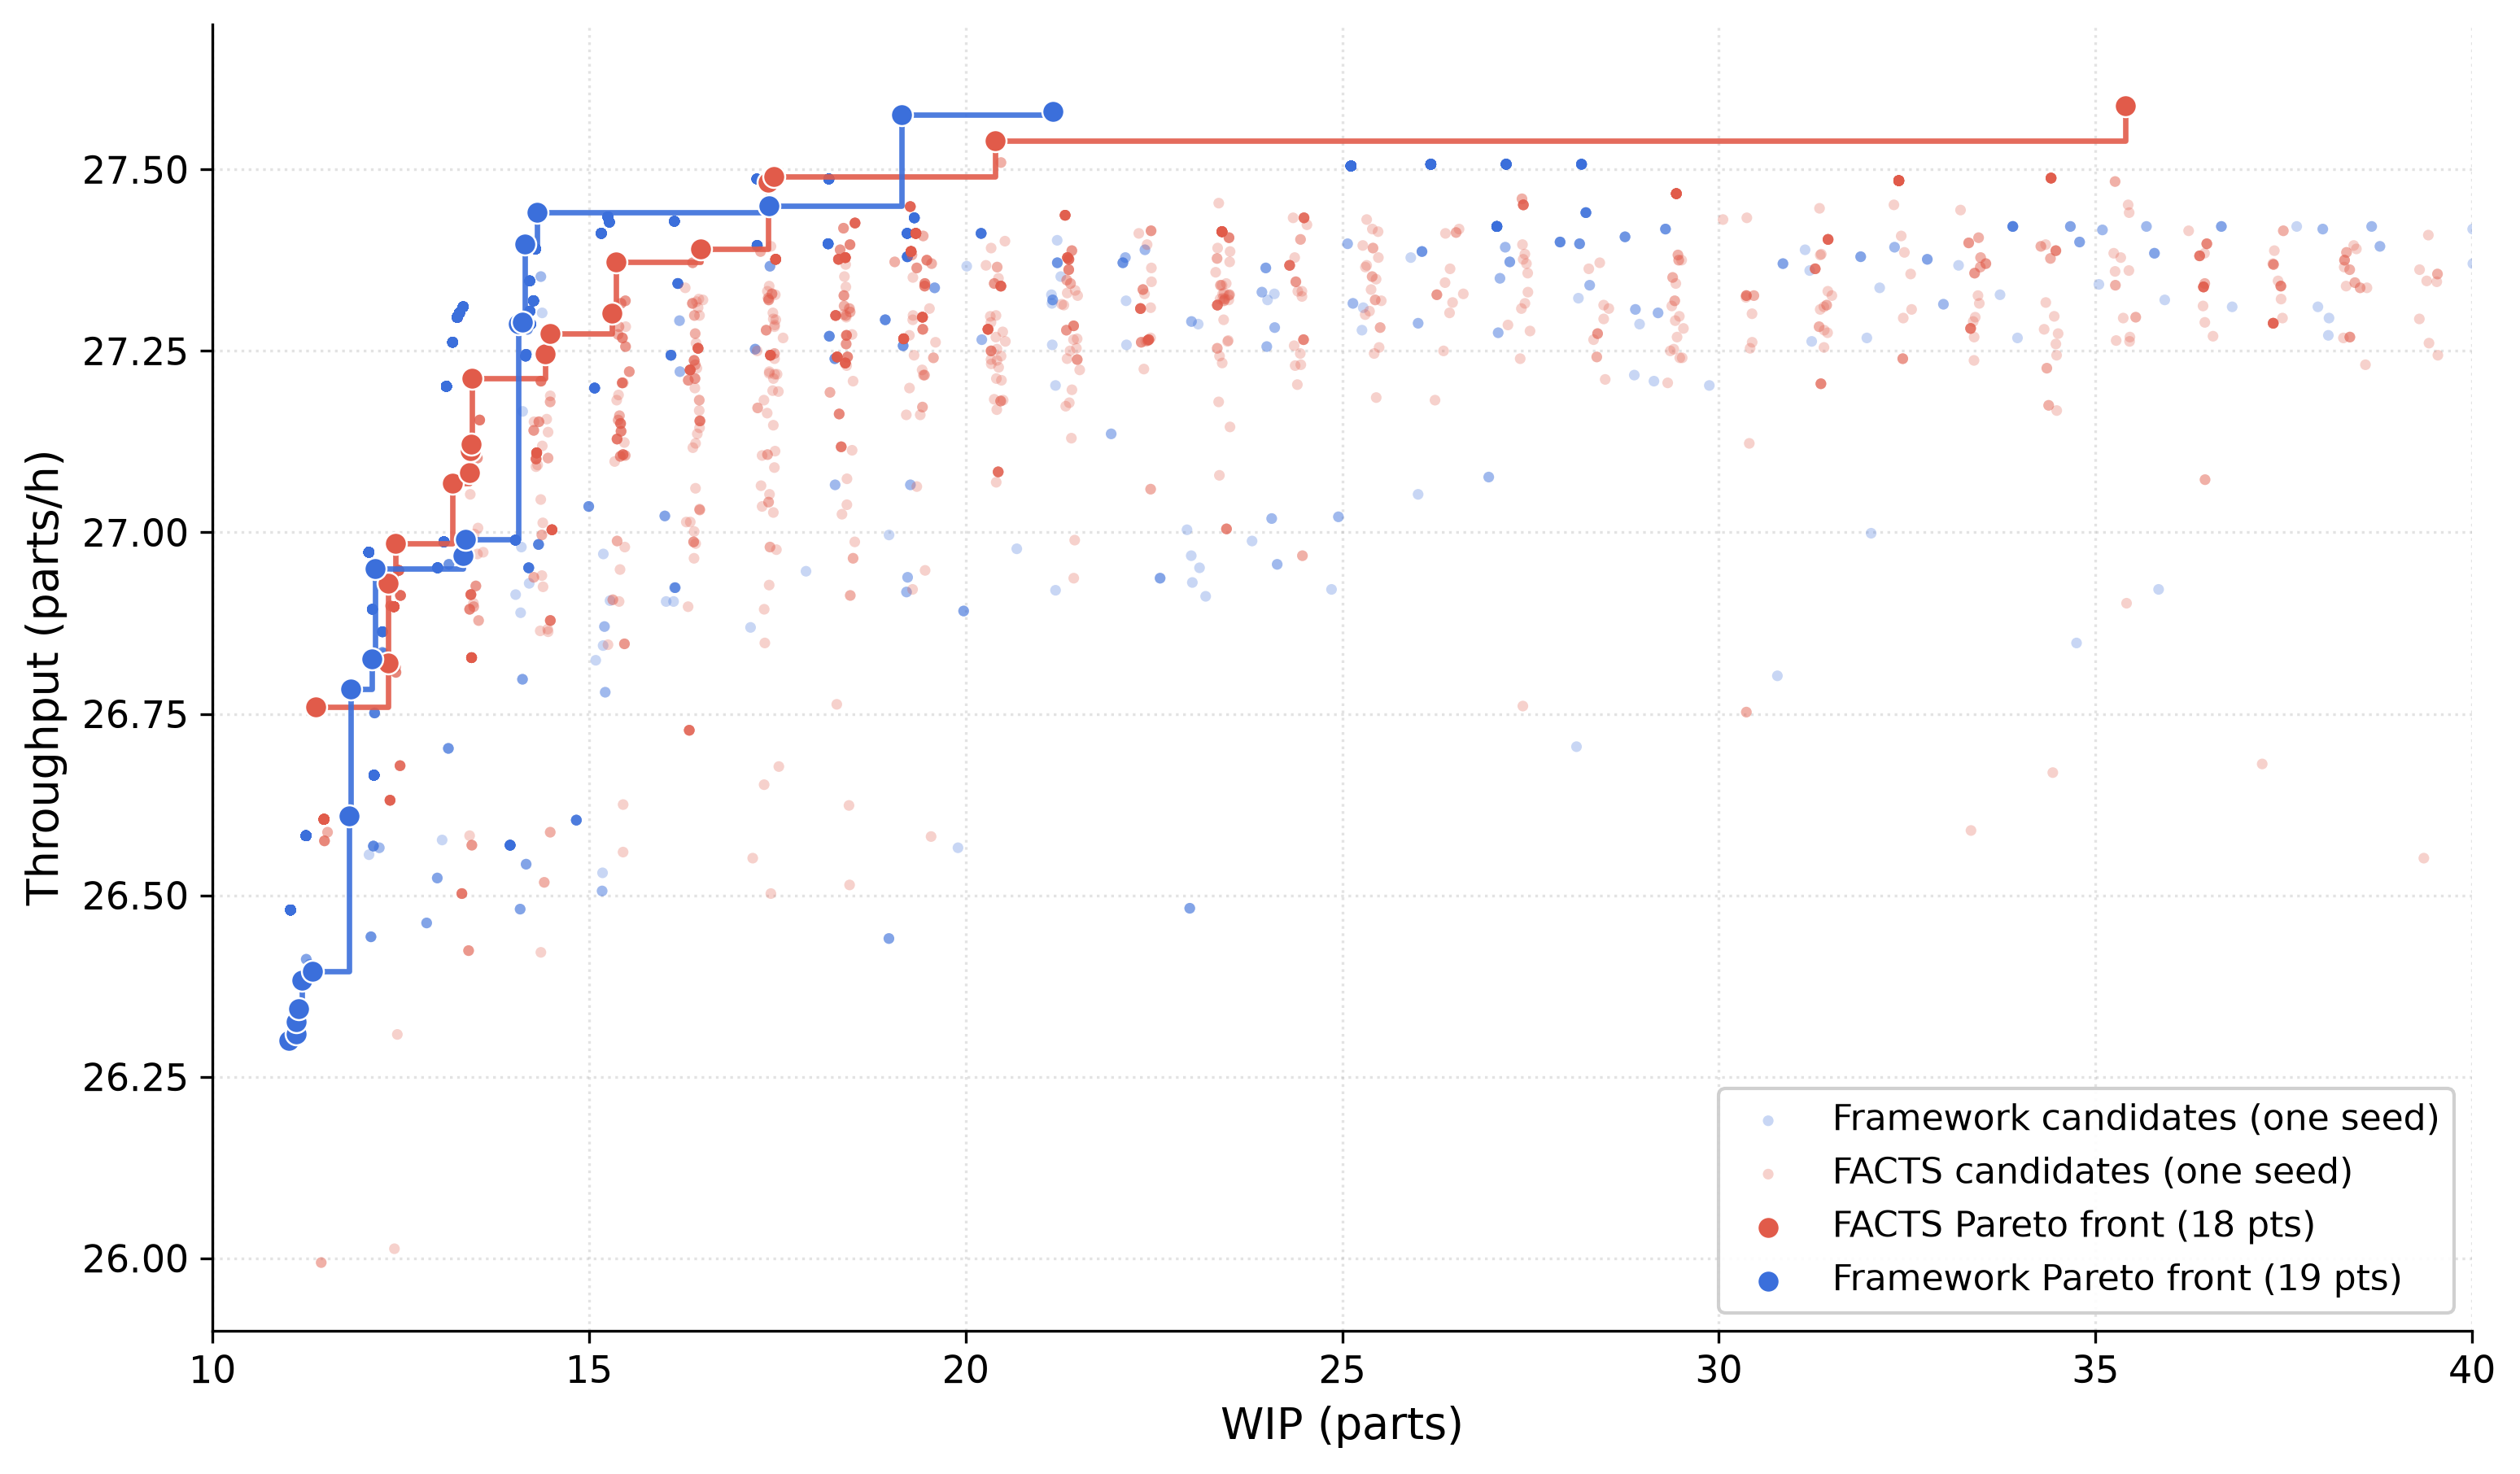
\includegraphics[width=0.75\textwidth]{figs/Fig4_TH_vs_WIP2.png}                                                   
  \caption{Solutions evaluated by the framework and by FACTS Analyzer for                                           
  Scenario~S1 (TH/WIP). Coloured dots are optimizer candidates from one                                             
  representative seed per optimizer; step lines are the corresponding                                               
  Pareto fronts. The Framework Pareto front is the 19-point front reported                                          
  in Table~\ref{tab:paretofront}. Coordinates of the three selected points                                          
  V1--V3 are listed in Table~\ref{tab:suggestions}.}                                                       
  \label{fig:MOEAdata}                                                                                              
  \end{figure}                                                                                                      
                                                                                                                    
  When re-simulated across ten random seeds with the canonical Python DES,                                          
  the three selected configurations yield the KPI deltas shown in                                                   
  Figure~\ref{fig:kpi-delta}. Relative to the unoptimized model                                                     
  (TH~$=27.15$~parts/h, WIP~$=18.16$~parts;                                                                         
  Table~\ref{tab:facts_python_comparison}), the lowest-WIP configuration                                            
  V1 reduces WIP by $38.6$~\% at the cost of $3.7$~\% of TH, and the                                                
  knee-point V2 reduces WIP by $22.2$~\% with essentially no loss of TH                                             
  (less than $0.3$~\%). The highest-TH configuration V3 recovers                                                    
  essentially the entire throughput of the unoptimized line ($+0.4$~\%                                              
  relative to Initial) at the cost of a $15.5$~\% \emph{increase} in WIP,                                           
  illustrating the TH/WIP trade-off that the Pareto front makes explicit.                                           
                                                                                                                    
  \begin{figure}[ ]                                                                                              
  \centering                                                                                                        
  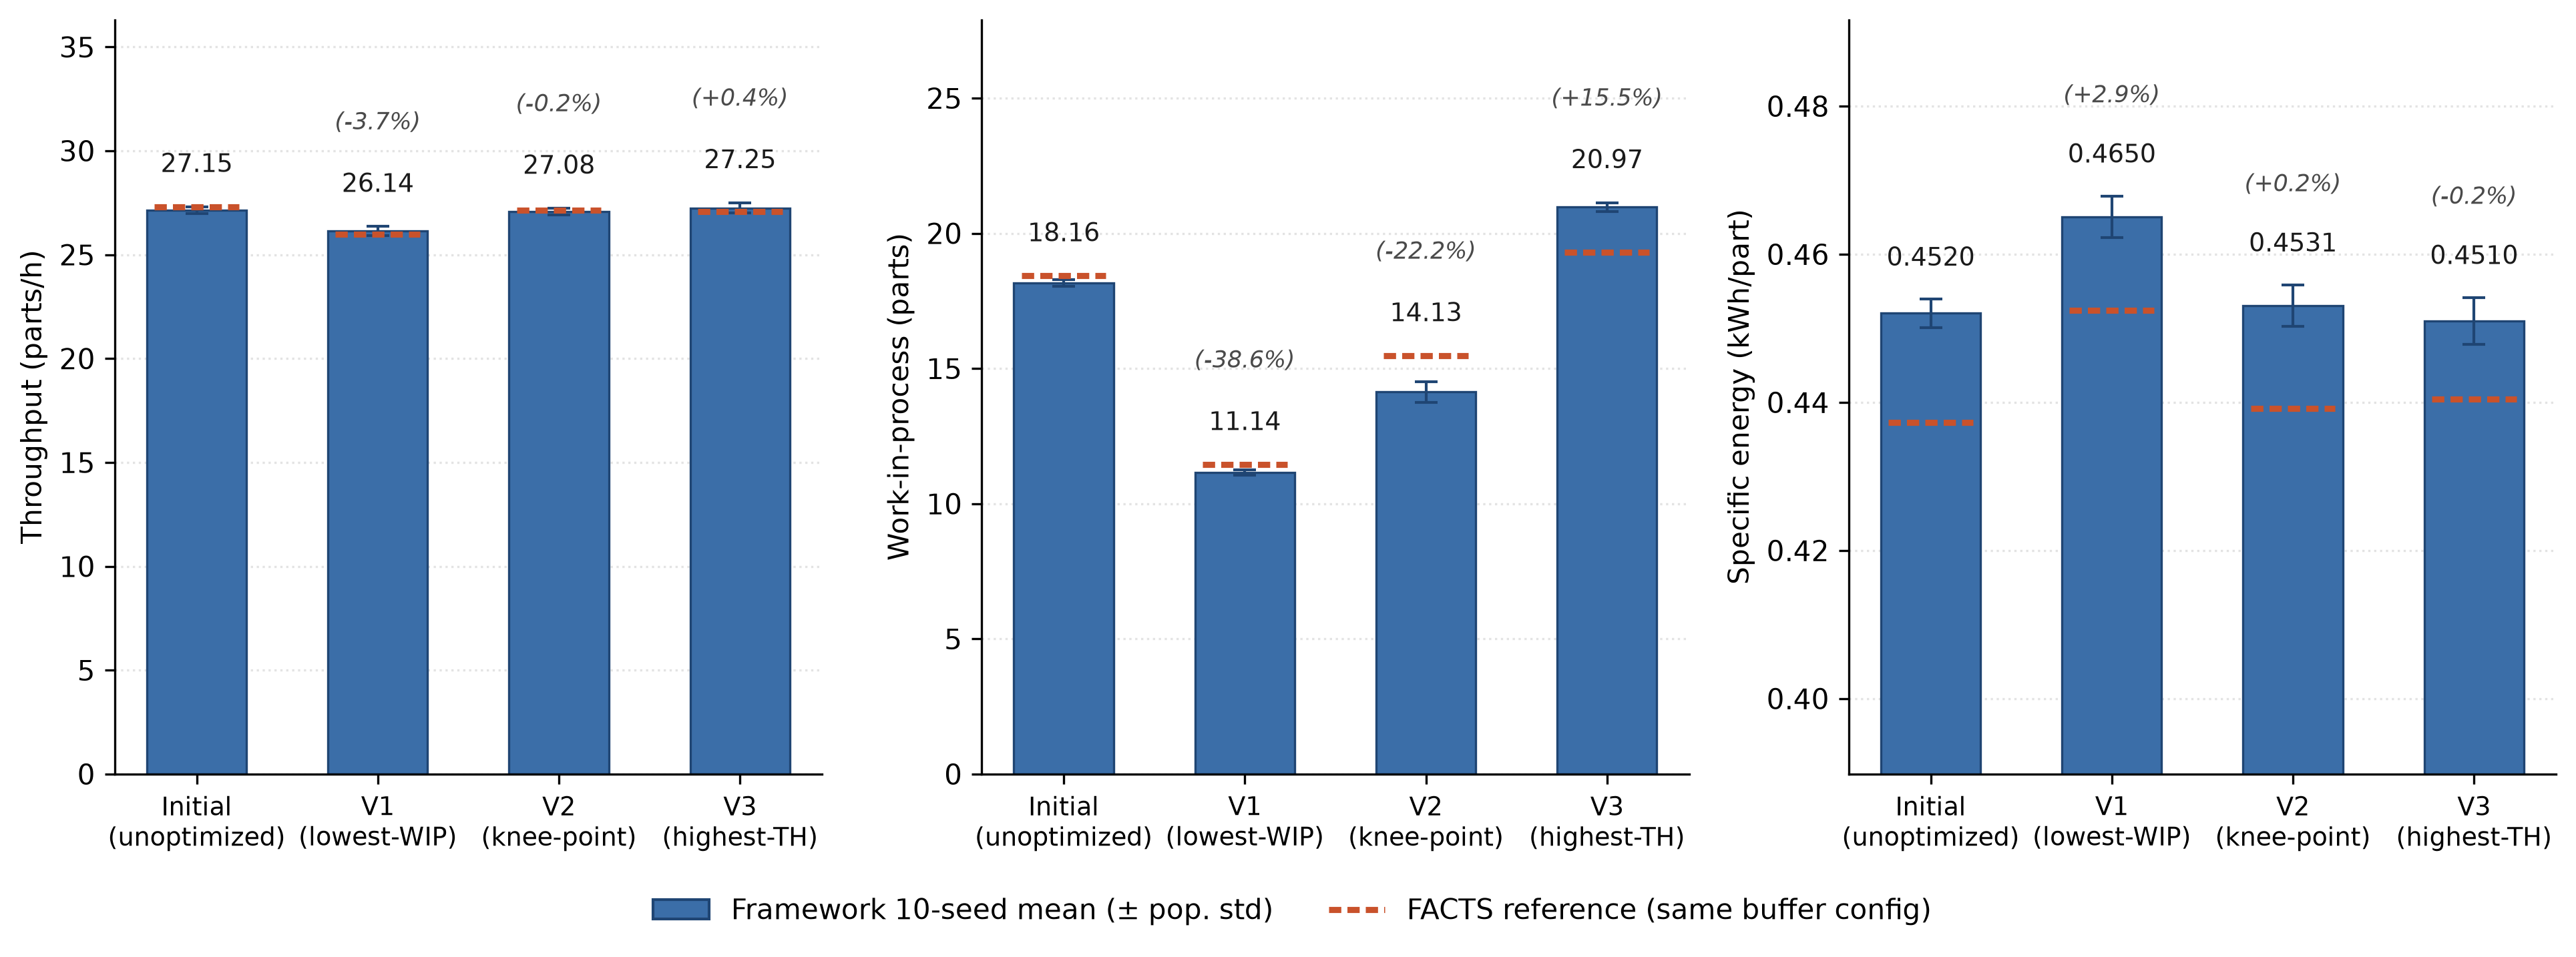
\includegraphics[width=0.85\textwidth]{figs/model_comparison_kpis2.png}                                            
  \caption{Ten-seed mean KPIs of the unoptimized model and of the three                                             
  adapted variants V1--V3 corresponding to the LLM-selected Pareto points                                           
  of Table~\ref{tab:suggestions}. Bars show the Framework 10-seed mean                                              
  ($\pm$ population standard deviation, error caps). Dashed orange markers                                          
  indicate the FACTS reference value for the same buffer configuration.                                             
  Italic percentages above each bar are the delta of the Framework mean                                             
  relative to the Initial (unoptimized) Framework mean.}                                                            
  \label{fig:kpi-delta}                                                                                             
  \end{figure}                                                                                                      
                                                                                                                    
                                                                 
                                                                                                            

   
  %For Scenario~S1 (TH/WIP), the framework returns a Pareto front with 16 non-dominated buffer configurations            
  %(Table~\ref{tab:paretofront}). Three points were selected from the front in response to a ``best balance between WIP and throughput'' user prompt at the HITL checkpoint~H5: the lowest-WIP corner, a knee-point, and the highest-TH corner(Table~\ref{tab:suggestions}). Figure~\ref{fig:MOEAdata} superimposes the framework's Pareto front on the FACTSAnalyzer reference front. The hypervolume of the framework's front, computed against the nadir $(\mathrm{WIP}=59.4,\mathrm{TH}=22.6)$ defined in Section~\ref{sec:case-evaluation}, is $235.53 \pm 1.63$ across ten seeds, against $233.98 \pm 1.00$ for the FACTS reference on the same nadir ($+0.66$~\%). Wilcoxon rank-sum test on the per-seed HV values gives $p = \TODO{fill from the released per-seed HV table}$, indicating that the framework matches the FACTS reference in the sense of statistical parity on this scenario.

  %\begin{table}[ ]                                                                                                  
  %\centering
  %\caption{Pareto front returned by the framework for Scenario~S1 (TH/WIP) on Case~A. Buf~1--6 are the six intermediate 
  %buffer capacities.}                                                                                                   
 % \label{tab:paretofront}                                                                                               
 % \csvreader[                                                                                                           
%      column names={                                                                                                    
%          generation_index = \genIdx,                                            %                                       
%          individual_index = \indIdx,                                                                                   
%          PostLoadingBuffer_capacity = \capA,                                                                           
%          PostConveyorBuffer_capacity = \capB,                                                                          
%          PostWashingBuffer_capacity = \capC,                                                                           
%          PrePress1Buffer_capacity = \capD,                                                                             
%          PrePress2Buffer_capacity = \capE,                                                                             
%          PostPress1_2_Buffer_capacity = \capF,                                  %                                       
%          total_buffer_capacity = \capTotal,                                      %                                      
%          wip = \valWip,                                                                                                
%          throughput = \valTp                                                                                           
%      },                                                                                                                
%      tabular={c c | c c c c c c | c | c r},                                                                            
%      table head=\toprule                                                                                               
%          \textbf{Gen.} & \textbf{Ind.} & \textbf{Buf 1} & \textbf{Buf 2} & \textbf{Buf 3} & \textbf{Buf 4} &           
%  \textbf{Buf 5} & \textbf{Buf 6} & \textbf{Total} & \textbf{WIP} & \textbf{TH} \\ \midrule,                            
%      late after line=\\,                                                                                               
%      table foot=\bottomrule                                                                                            
%  ]{figs/moo_pareto_solutions.csv}{}{%                                                                                  
%      \genIdx & \indIdx & \capA & \capB & \capC & \capD & \capE & \capF & \capTotal & \num[round-mode=places,           
%  round-precision=2]{\valWip} & \num[round-mode=places, round-precision=2]{\valTp}                                      
%  }                                                                                                                     
%  \end{table}                                                                                                           
                                                            
%  \begin{table}[ ]                                                                                                  
%  \centering                                                
%  \caption{Three Pareto points selected at HITL checkpoint~H5 for further evaluation.}                                  
%  \label{tab:suggestions}                                                                                               
%  \csvreader[                                                                                                           
%      column names={                                                                                                    
%          PostLoadingBuffer_capacity = \capA,                                                                           
%          PostConveyorBuffer_capacity = \capB,                                                                          
%          PostWashingBuffer_capacity = \capC,                                                                           
%          PrePress1Buffer_capacity = \capD,                                                                             
%          PrePress2Buffer_capacity = \capE,                                                                             
%          PostPress1_2_Buffer_capacity = \capF,                                   %                                      
%          total = \capTotal,                                                                                            
%          wip = \valWip,                                                                                                
%          throughput = \valTp                                                                                           
%      },                                                                                                                
%      tabular={c c c c c c | c | c r},                                                                                  
%      table head=\toprule                                                                                               
%          \textbf{Buf 1} & \textbf{Buf 2} & \textbf{Buf 3} & \textbf{Buf 4} & \textbf{Buf 5} & \textbf{Buf 6} &         
%  \textbf{Total} & \textbf{WIP} & \textbf{TH} \\ \midrule,                                                              
%      late after line=\\,                                                                                               
%      table foot=\bottomrule                                                                                            
%  ]{figs/suggested_improvements_fix.csv}{}{%                                                                            
%      \capA & \capB & \capC & \capD & \capE & \capF & \capTotal & \num[round-mode=places, round-precision=2]{\valWip} & 
%  \num[round-mode=places, round-precision=2]{\valTp}                                                                    
%  }                                                                                                                     
%  \end{table}                                                                                                           
                                                                                                                        
\subsection{Automated SCORE bottleneck analysis}\label{sec:results-bn}                                                                    
                                         
  The automated SCORE analysis (Stage~S4) identifies the two press cells as                                                                 
  the dominant bottlenecks in Case~A, in agreement with practitioner
  intuition and with the FACTS Analyzer SCORE setup. The framework's top-four                                                               
  alleviation actions -- reduce the process time of Presses cell~2 and                                                                      
  Presses cell~1 by 10~\%, and increase the availability of Presses cell~2                                                                  
  and Presses cell~1 by 10~\% -- coincide as an unordered set with the                                                                      
  top-four bars of the FACTS SCORE ranking (Figure~\ref{fig:SCORE}); only the                                                               
  intra-pair ordering of the two availability actions differs between the                                                                   
  two rankings. At rank five the two rankings diverge on the same machine:                                                                  
  the framework prioritizes reducing the Washing Machine's process time,                                                                    
  whereas the FACTS SCORE ranks the Washing Machine's availability first.                                                                   
  This rank-five discrepancy is attributable to MOEA stochasticity, and the                                                                 
  FACTS setup itself fluctuates between rank-5 candidates across reruns.                                                                    
  Each alleviation action is accompanied by a short natural-language                                                                        
  explanation generated by the bottleneck agent; practitioners at the host                                                                  
  company singled these explanations out as the most immediately useful                                                                     
  artifact of the framework                                                                                                                 
  (Section~\ref{sec:discussion-industry}).                                                                                                  
                                                                                                                                            
  \begin{figure}[]                                                                                                                      
    \centering                                                                                                                              
    \begin{subfigure}{0.42\textwidth}                                                                                                       
      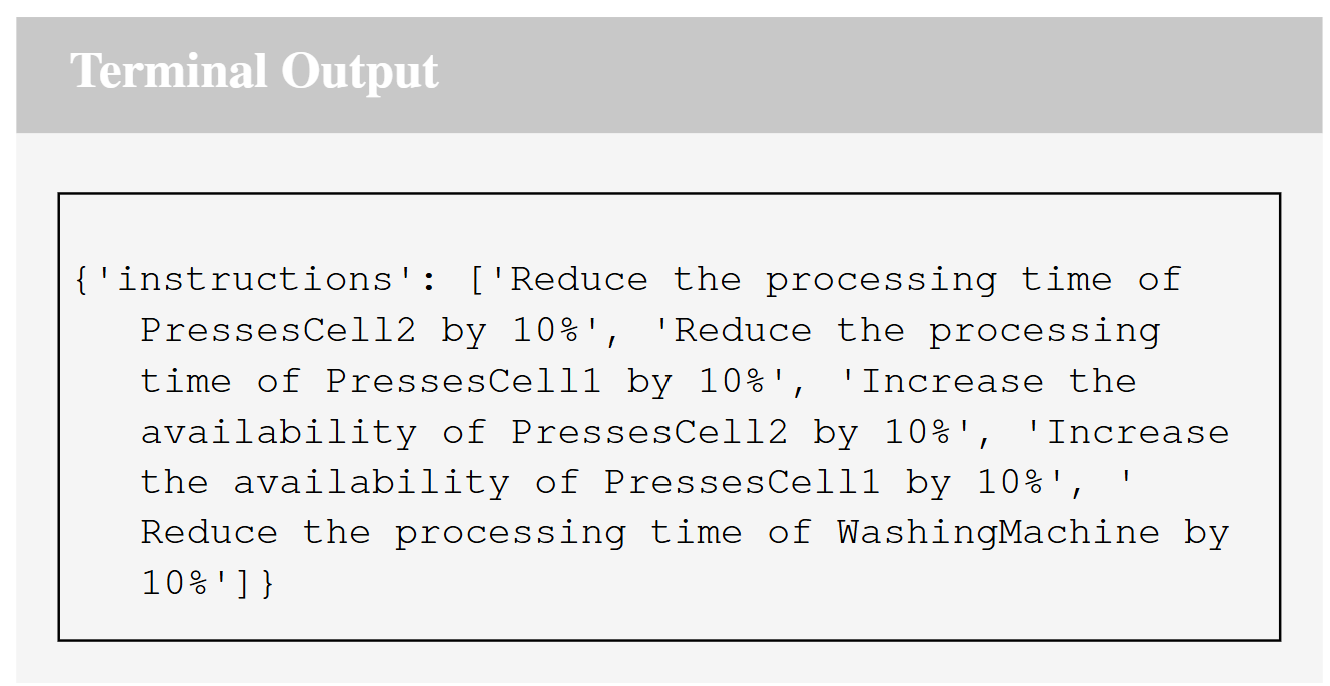
\includegraphics[width=\textwidth]{figs/bottleneckinstructions.png}                                                                   
      \label{fig:SCORE-top}                                                                                                                 
    \end{subfigure}                                                                                                                         
    \vspace{1em}                                                                                                                            
    \begin{subfigure}{0.42\textwidth}                                                                                                       
      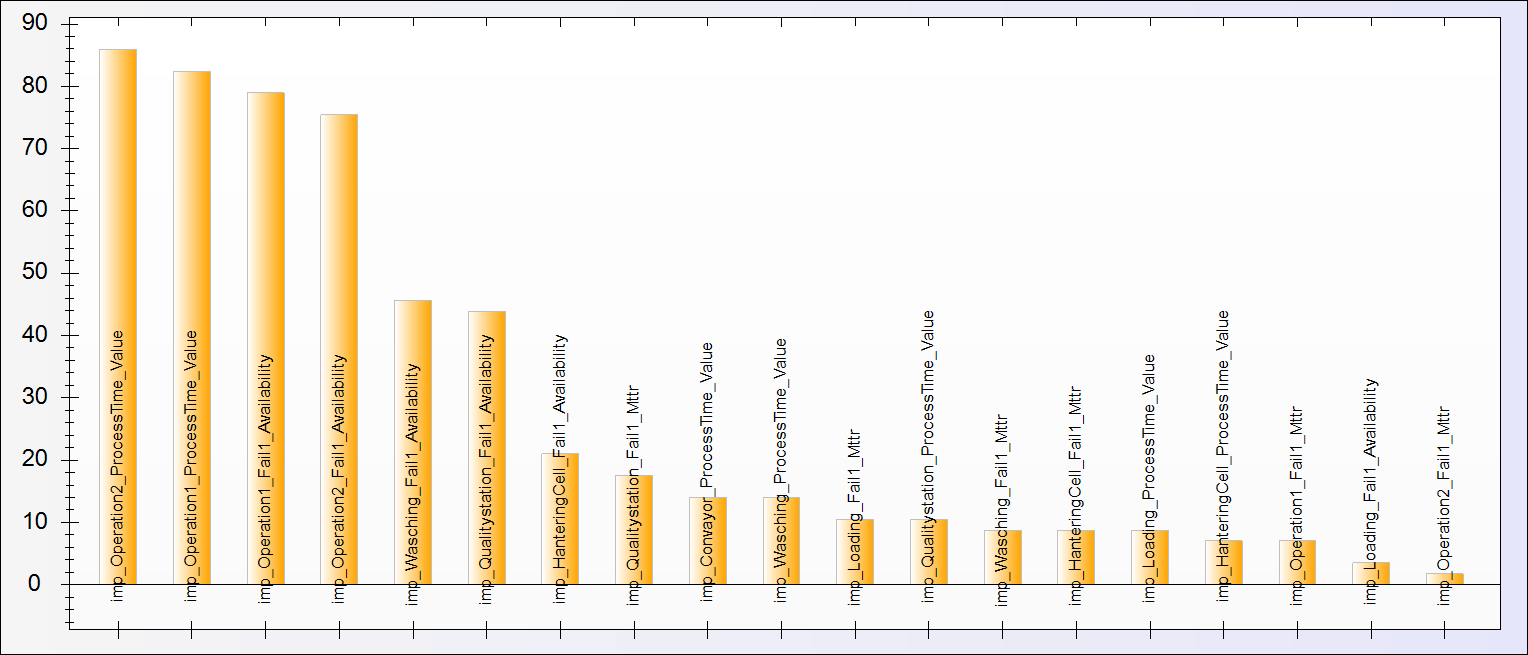
\includegraphics[width=\textwidth]{figs/FACTS_SCORE_bottleneck_scenario.png}                                                          
      \label{fig:SCORE-bottom}                                                                                                              
    \end{subfigure}                                                                                                                         
    \caption{Top alleviation actions identified by the framework's automated                                                                
    SCORE analysis (top: terminal output of the bottleneck agent) and by the                                                                
    FACTS Analyzer SCORE setup (bottom: relative-frequency bar chart over                                                                   
    the non-dominated SCORE solutions). The four highest-ranked actions                                                                     
    -- reducing process time and increasing availability of the two press                                                                   
    cells -- coincide as an unordered set between the two optimizers;                                                                       
    ranking at position five differs on the Washing Machine variable and is                                                                 
    discussed in the text.}                                                                                                                 
    \label{fig:SCORE}                                                                                                                       
  \end{figure}                                                                                                                              
                                                                                                                                            
  To assess the framework's response to what-if follow-up questions, five                                                                   
  alleviation scenarios were tested on the dominant Presses cell~2                                                                          
  bottleneck, each re-simulated across the ten baseline seeds                                                                               
  $\{11, 22, \ldots, 110\}$ on the unoptimized DES with the canonical                                                                       
  released Python DES: (a)~a 10~\% reduction in cycle time (process time                                                                    
  $\times 0.9$); (b)~a 10~pp increase in availability (from 87.69~\% to                                                                     
  97.69~\%); (c)~a 10~\% reduction in MTTR (MTTR $\times 0.9$); (d)~doubling                                                                
  the buffer immediately upstream of the press (PrePress2 capacity                                                                          
  $3 \to 6$); and (e)~doubling the buffer immediately downstream                                                                            
  (PostPress1--2 capacity $3 \to 6$). Relative to the unoptimized baseline                                                                  
  (TH~$=27.15$~parts/h, WIP~$=18.16$~parts;                                                                                                 
  Table~\ref{tab:facts_python_comparison}), reducing cycle time (a) and                                                                     
  increasing availability (b) raise TH by $5.7$~\% and $5.9$~\% respectively                                                                
  with limited change in WIP. MTTR reduction (c) yields a much smaller                                                                      
  TH gain of $0.24$~\%, because a 10~\% MTTR reduction on this machine                                                                      
  translates to only a ${\sim}1$~pp effective availability increase and                                                                     
  therefore has an order-of-magnitude smaller impact than direct                                                                            
  availability alleviation (b). Doubling the upstream buffer (d) raises                                                                     
  WIP by $16.3$~\% without measurable TH gain, and doubling the downstream                                                                  
  buffer (e) yields no measurable change in either KPI, consistent with the                                                                 
  bottleneck agent's textual explanation that the press is rarely blocked                                                                   
  downstream. 


\subsection{Component ablation}\label{sec:results-ablation}                                                                               
              
  To isolate the contribution of each component of the framework, eight                                                                     
  ablation configurations were evaluated on Case~A, in addition to the
  FACTS reference. Each configuration was run for ten independent seeds.                                                                    
  The four axes examined are: the two blueprints (simulation, MOO), the                                                                    
  inspector agent, the LLM tier (GPT-5-mini, GPT-5-nano), and the sampling                                                                  
  temperature ($T \in \{0.0, 0.7, 1.0\}$).                                                                                                  
  Tables~\ref{tab:ablation_kpi_comparison_extended}--\ref{tab:ablation_errors}                                                              
  report the resulting KPI fidelity, hypervolume, cost, and error counts.                                                                   
                                                                                                                                            
  Note that the KPI columns in                                                                                                              
  Table~\ref{tab:ablation_kpi_comparison_extended} and the per-seed values                                                                  
  in Table~\ref{tab:seed_metrics} are computed from the ten LLM-generated                                                                   
  per-seed initial-model runs and therefore report variability across LLM                                                                   
  code generations, whereas Table~\ref{tab:facts_python_comparison} in                                                                      
  Section~\ref{sec:results-fidelity} reports fidelity of the canonical                                                                      
  released Python DES across ten random seeds. This distinction explains                                                                    
  why the two ``Framework Initial'' means differ slightly                                                                                   
  ($27.298$~parts/h in Table~\ref{tab:ablation_kpi_comparison_extended}                                                                     
  vs.\ $27.15$~parts/h in Table~\ref{tab:facts_python_comparison}).                                                                         
                                                                                                                                            
  \begin{table}[]                                                                                                                       
  \centering                                                                                                                                
  \caption{KPI fidelity per ablation configuration, averaged over the ten                                                                   
  seeds per configuration (LLM-generated per-seed initial-model runs).                                                                      
  ``Feasible runs'' is the number of seeds (out of ten) whose initial-model                                                                 
  KPIs were within an acceptable range; degenerate model-build failures                                                                     
  (e.g.\ seed~88 in the Baseline) are excluded from the averaged KPI columns.                                                               
  FACTS is the reference; percentage deltas are relative to FACTS.}                                                                         
  \label{tab:ablation_kpi_comparison_extended}                                                                                              
  \begin{tabular}{@{}l c r r r@{}}                                                                                                          
  \toprule                                                                                                                                  
  \textbf{Configuration} & \textbf{Feasible runs} & \textbf{TH vs FACTS avg} & \textbf{WIP vs FACTS avg} & \textbf{SEC vs FACTS avg} \\     
  \midrule                                                                                                                                  
  FACTS (reference)     & 10 & 27.31 ($0$\%)       & 18.43 ($0$\%)       & 0.4373 ($0$\%)      \\                                           
  Baseline              & 9  & 27.298 ($-0.045$\%) & 18.161 ($-1.459$\%) & 0.4532 ($+3.628$\%) \\                                           
  No simulation bp.     & 0  & --                  & --                  & --                  \\                                           
  No MOO blueprint      & 10 & 27.305 ($-0.018$\%) & 18.155 ($-1.492$\%) & 0.4531 ($+3.609$\%) \\                                           
  No inspector          & 10 & 27.241 ($-0.253$\%) & 18.061 ($-2.002$\%) & 0.4536 ($+3.718$\%) \\                                           
  GPT-5-mini            & 10 & 27.232 ($-0.286$\%) & 18.059 ($-2.013$\%) & 0.4539 ($+3.789$\%) \\                                           
  GPT-5-nano            & 6  & 27.268 ($-0.153$\%) & 18.125 ($-1.655$\%) & 0.4535 ($+3.708$\%) \\                                           
  $T=0.0$               & 10 & 27.328 ($+0.066$\%) & 18.154 ($-1.497$\%) & 0.4528 ($+3.556$\%) \\                                           
  $T=0.7$               & 9  & 27.270 ($-0.147$\%) & 18.104 ($-1.766$\%) & 0.4532 ($+3.626$\%) \\                                           
  $T=1.0$               & 9  & 27.299 ($-0.041$\%) & 18.176 ($-1.381$\%) & 0.4532 ($+3.631$\%) \\                                           
  \bottomrule                                                                                                                               
  \end{tabular}                                                                                                                             
  \end{table}                                                                                                                               
                                                                                                                                            
  \begin{table}[]                                                                                                                       
  \centering                                                                                                                                
  \caption{Optimization quality per ablation configuration. HV is computed                                                                  
  against the common nadir $(\mathrm{WIP}=59.4, \mathrm{TH}=22.6)$.                                                                         
  ``Completed MOO'' is the number of runs (out of ten) in which the LLM                                                                     
  pipeline finished the MOEA stage; ``Feasible MOO'' is the number of those                                                                 
  runs whose Pareto front was usable for the hypervolume computation.                                                                       
  $\Delta$ HV and HV std are computed across the feasible MOO runs.}                                                                        
  \label{tab:ablation_difference}                                                                                                           
  \begin{tabular}{@{}l c c c c r c@{}}                                                                                                      
  \toprule                                                                                                                                  
  \textbf{Configuration} & \textbf{Completed MOO} & \textbf{MOO time avg (s)} & \textbf{Feasible MOO} & \textbf{HV avg} & \textbf{$\Delta$  
  HV vs FACTS} & \textbf{HV std} \\                                                                                                         
  \midrule                                                                                                                                  
  FACTS (reference)     & 10 & 625   & 10 & 233.98 & $0$\%       & 1.00 \\                                                                  
  Baseline              & 10 & 815   & 9  & 235.53 & $+0.66$\%   & 1.63 \\                                                                  
  No simulation bp.     & 8  & 1562  & 0  & --     & --          & --   \\                                                                  
  No MOO blueprint      & 4  & 2423  & 3  & 239.77 & $+2.47$\%   & 10.29 \\                                                                 
  No inspector          & 7  & 469   & 7  & 234.05 & $+0.03$\%   & 1.54 \\                                                                  
  GPT-5-mini            & 10 & 226   & 10 & 232.68 & $-0.56$\%   & 7.94 \\                                                                  
  GPT-5-nano            & 9  & 482   & 0  & --     & --          & --   \\                                                                  
  $T=0.0$               & 10 & 358   & 10 & 234.21 & $+0.10$\%   & 2.03 \\                                                                  
  $T=0.7$               & 10 & 384   & 9  & 232.77 & $-0.52$\%   & 1.94 \\                                                                  
  $T=1.0$               & 8  & 533   & 7  & 233.04 & $-0.40$\%   & 2.29 \\                                                                  
  \bottomrule                                                                                                                               
  \end{tabular}                                                                                                                             
  \end{table}                                                                                                                               
                                                                                                                                            
  \begin{table}[]                                                                                                                       
  \centering                                                                                                                                
  \caption{Operational cost per ablation configuration. Wall-clock time is                                                                  
  dominated by DES evaluations; the LLM-call count and token totals are                                                                     
  strongly bounded by the pipeline structure. ``Completed runs'' is the                                                                     
  number of seeds (out of ten) whose full pipeline finished end-to-end.}                                                                    
  \label{tab:ablation_performance}   
  \resizebox{\textwidth}{!}{%
  \begin{tabular}{@{}l c c c c c c@{}}                                                                                                      
  \toprule                                                                                                                                  
  \textbf{Configuration} & \textbf{Completed runs} & \textbf{Wall-clock avg (s)} & \textbf{LLM calls avg} & \textbf{Input tok.\ avg} &      
  \textbf{Output tok.\ avg} & \textbf{Cost avg (USD)} \\                                                                                    
  \midrule                                                                                                                                  
  Baseline              & 10 & 992  & 14.1 & 62{,}278 & 45{,}918 & 0.319 \\                                                                 
  No simulation bp.     & 3  & 2362 & 14.0 & 44{,}445 & 36{,}966 & 0.243 \\                                                                 
  No MOO blueprint      & 3  & 3683 & 14.0 & 58{,}219 & 44{,}495 & 0.303 \\                                                                 
  No inspector          & 7  & 872  & 12.0 & 50{,}635 & 39{,}143 & 0.204 \\                                                                 
  GPT-5-mini            & 10 & 918  & 14.3 & 65{,}723 & 60{,}819 & 0.136 \\                                                                 
  GPT-5-nano            & 4  & 1142 & 14.0 & 60{,}595 & 96{,}377 & 0.038 \\                                                                 
  $T=0.0$               & 10 & 786  & 14.0 & 62{,}020 & 45{,}887 & 0.316 \\                                                                 
  $T=0.7$               & 10 & 863  & 14.0 & 63{,}191 & 47{,}138 & 0.324 \\                                                                 
  $T=1.0$               & 8  & 1191 & 14.4 & 66{,}185 & 49{,}708 & 0.356 \\                                                                 
  \bottomrule                                                                                                                               
  \end{tabular} 
  }
  \end{table}                                                                                                                               
                                                                                                                                            
  \begin{table}[]                                                                                                                       
  \centering                                                                                                                                
  \caption{Total error events per configuration over the ten runs. Because                                                                  
  the inspector agent iterates on failing code, a single run may generate                                                                   
  several syntax or structural errors before the code passes; the counts                                                                    
  are therefore \emph{event counts}, not run counts. Reasoning errors were                                                                  
  labelled by manual inspection of the runs.}                                                                                               
  \label{tab:ablation_errors}                                                                                                               
  \begin{tabular}{@{}l c c c@{}}                                                                                                            
  \toprule                                                                                                                                  
  \textbf{Configuration} & \textbf{Syntax errors} & \textbf{Structural errors} & \textbf{Reasoning errors} \\                               
  \midrule                                                                                                                                  
  Baseline              & 0  & 2  & 4 \\                                                                                                    
  No simulation bp.     & 20 & 19 & 0 \\                                                                                                    
  No MOO blueprint      & 8  & 7  & 0 \\                                                                                                    
  No inspector          & 3  & 2  & 1 \\                                                                                                    
  GPT-5-mini            & 3  & 2  & 7 \\                                                                                                    
  GPT-5-nano            & 7  & 11 & 0 \\                                                                                                    
  $T=0.0$               & 0  & 0  & 4 \\                                                                                                    
  $T=0.7$               & 0  & 3  & 4 \\                                                                                                    
  $T=1.0$               & 2  & 4  & 3 \\                                                                                                    
  \bottomrule                                                                                                                               
  \end{tabular}                                                                                                                             
  \end{table}                                                                                                                               
                                                                                                                                            
  Three findings emerge. First, the simulation and MOO blueprints                                                                           
  materially reduce structural errors: removing the simulation blueprint                                                                    
  eliminates every feasible MOO run (Feasible MOO drops to $0$ of ten in                                                                    
  Table~\ref{tab:ablation_difference}), and removing the MOO blueprint                                                                      
  reduces MOO feasibility from nine to three of ten seeds. Second, the                                                                      
  inspector agent salvages the majority of remaining failures without                                                                       
  practitioner involvement; disabling it reduces the number of completed                                                                    
  runs from ten to seven (Table~\ref{tab:ablation_performance}) and does                                                                    
  not materially affect HV on the runs that do complete                                                                                     
  ($234.05$ vs.\ $235.53$ for the Baseline, within one HV std).                                                                             
  Third, downgrading the model tier from GPT-5.1 to GPT-5-mini preserves                                                                    
  the baseline HV within statistical noise ($232.68$ vs.\ $235.53$,                                                                         
  i.e.\ within roughly two Baseline HV stds) while reducing cost by roughly                                                                 
  a factor of $2.3$ in absolute terms ($0.319$ to $0.136$ USD per completed                                                                 
  study), whereas GPT-5-nano generates syntactically valid code but never                                                                   
  produces a feasible MOO artifact (Feasible MOO $= 0$). In practical                                                                       
  deployment terms, GPT-5-mini is the recommended production tier for                                                                       
  cost-sensitive settings.                                                                                                                  
                                                                                                            
                                                                                                                                        








  \subsection{Operational cost}\label{sec:results-cost}                                                                 
  
  A representative baseline run of the framework consumes on average $62{,}278$ input tokens and $45{,}918$ output      
  tokens across roughly 14 LLM calls, at an OpenAI API cost of approximately USD~0.319 per completed study
  (Table~\ref{tab:seed_metrics}). Inputs account for about 58~\% of total tokens. End-to-end wall-clock time is         
  dominated by simulation runs rather than by LLM calls: the DES budget scales linearly with population size,
  generations, and simulation horizon, whereas the number of LLM calls is bounded by the number of pipeline stages and
  is essentially independent of problem size.

  \begin{table}[ ]                                                                                                  
  \centering
  \caption{Baseline per-seed metrics for the framework on Case~A. Seed~88 is a known model-build failure (see           
  \S~\ref{sec:results-fidelity}) and is excluded from the HV averages reported in \S~\ref{sec:results-moo}.}            
  \label{tab:seed_metrics}
  \resizebox{\textwidth}{!}{%
  \begin{tabular}{@{}c c c c c c c c c c c@{}}                                                                          
  \toprule                                                                                                              
  \textbf{Seed} & \textbf{TH} & \textbf{WIP} & \textbf{SEC} & \textbf{MOO time (s)} & \textbf{HV} & \textbf{Total time  
  (s)} & \textbf{Input tok.} & \textbf{Output tok.} & \textbf{Cost (USD)} & \textbf{LLM calls} \\                       
  \midrule                                                                                                              
  11  & 27.25 & 18.18 & 0.4542 & 526 & 236.66 & 1052 & 64{,}666 & 46{,}759 & 0.33 & 14 \\                               
  22  & 27.24 & 18.15 & 0.4548 & 337 & 236.24 & 860  & 58{,}984 & 43{,}226 & 0.28 & 14 \\                               
  33  & 27.23 & 18.25 & 0.4541 & 537 & 233.76 & 1094 & 63{,}184 & 45{,}261 & 0.31 & 14 \\                               
  44  & 27.36 & 18.18 & 0.4519 & 245 & 235.07 & 737  & 62{,}873 & 46{,}209 & 0.32 & 14 \\                               
  55  & 27.34 & 18.16 & 0.4525 & 335 & 235.63 & 860  & 56{,}471 & 40{,}941 & 0.31 & 15 \\                               
  66  & 27.24 & 17.99 & 0.4547 & 682 & 238.07 & 1380 & 60{,}330 & 47{,}610 & 0.32 & 14 \\                               
  77  & 27.35 & 18.18 & 0.4522 & 420 & 235.13 & 1017 & 63{,}555 & 47{,}249 & 0.33 & 14 \\                               
  88  & 23.17 & 18.03 & 0.5102 & 572 & --      & 1009 & 64{,}114 & 46{,}823 & 0.33 & 14 \\                              
  99  & 27.32 & 18.17 & 0.4523 & 335 & 236.89 & 765  & 63{,}868 & 47{,}757 & 0.33 & 14 \\                               
  110 & 27.34 & 18.19 & 0.4518 & 663 & 232.32 & 1150 & 64{,}737 & 47{,}348 & 0.33 & 14 \\                               
  \bottomrule                                                                                                           
  \end{tabular} 
  }
  \end{table}                                                                                                           
                                                                
% ======================================================================                                                                  
  % 6. Performance retention under sustained parameter perturbations
  % ======================================================================                                                                  
  \section{Performance retention under sustained parameter perturbations}\label{sec:resilience}                                             
                                                                                                                                            
  Sections~\ref{sec:results-moo}--\ref{sec:results-bn} evaluate the                                                                         
  framework under nominal operating conditions. Industrial deployment,                                                                      
  however, also requires understanding how candidate solutions behave when                                                                  
  specific machine parameters deteriorate. We therefore perform a
  steady-state sensitivity analysis: the DES is stress-tested under                                                                         
  sustained parameter perturbations representing degraded operating states,                                                                 
  and the fraction of nominal throughput retained by each Pareto                                                                            
  configuration is quantified. We deliberately restrict attention to                                                                        
  sustained perturbations because the DES targets steady-state throughput                                                                   
  evaluation; transient disruption-and-recovery dynamics, recovery times,                                                                   
  and adaptation trajectories are outside the scope of the current model                                                                    
  and are discussed as future work in                                                                                                       
  Section~\ref{sec:discussion-limits}. Within these boundaries, the                                                                         
  analysis addresses one operational dimension of manufacturing                                                                             
  resilience -- namely, the retention of production performance under                                                                       
  sustained equipment or reliability degradation -- and does not claim to                                                                   
  model the full disruption-and-recovery process.                                                                                           
  Section~\ref{sec:res-r1} evaluates the performance retention of the                                                                       
  Pareto solutions returned by the MOEA under three perturbation                                                                            
  scenarios; Section~\ref{sec:res-r2} examines whether bottleneck                                                                           
  rankings remain stable across these conditions; and                                                                                       
  Section~\ref{sec:res-r3} quantifies the cost of answering a series of                                                                     
  sensitivity what-if queries.                                                                                                              
                                                                                                                                            
  \subsection{Perturbation scenarios and retention metric}\label{sec:res-scenarios}                                                         
                                                                                                                                            
  For a Pareto-optimal buffer configuration $x$ and a perturbation                                                                          
  scenario $d$, let $TH_\mathrm{nom}(x)$ denote the mean nominal
  throughput and $TH_d(x)$ the mean throughput under $d$, each averaged                                                                     
  over $n_\mathrm{seed}=5$ replications. Following the                                                                                      
  retention-of-performance perspective reviewed by                                                                                          
  \citet{Hosseini2016}, we define the \emph{worst-case                                                                                      
  performance-retention score}                                                                                                              
                                                                                                                                            
  \begin{equation}                                                                                                                          
  R_\mathrm{worst}(x)                                                                                                                       
  =                                                                                                                                         
  \min_{d \in \{D_1,D_2,D_3\}}                              
  \frac{TH_d(x)}{TH_\mathrm{nom}(x)}.                                                                                                       
  \end{equation}                                                                                                                            
                                                                                                                                            
  $R_\mathrm{worst}(x)=1$ denotes a configuration whose throughput is                                                                       
  fully retained under all three sustained perturbations considered;                                                                        
  lower values indicate greater sensitivity to degraded operating                                                                           
  conditions. We interpret this quantity as a measure of operational                                                                        
  performance retention -- and therefore as one component of manufacturing                                                                  
  resilience -- rather than as a comprehensive resilience metric. In                                                                        
  particular, the present analysis does not capture recovery time,                                                                          
  adaptation trajectories, or restoration following a transient                                                                             
  disruption. Because the scenarios considered here are modelled as                                                                         
  sustained parameter perturbations, a retention-of-performance                                                                             
  formulation is appropriate; time-integrated measures such as the                                                                          
  ``resilience triangle'' of \citet{Bruneau2003} are more appropriate when                                                                  
  performance degradation and subsequent recovery are explicitly modelled.                                                                  
                                                                                                                                            
  The three perturbation scenarios are summarized in                                                                                        
  Table~\ref{tab:res_scenarios}; each targets a topologically distinct                                                                      
  part of the line, and their magnitudes were calibrated so that the                                                                        
  resulting throughput impact discriminates between Pareto solutions                                                                        
  rather than saturating the response.                                                                                                      
                                                                                                                                            
  \begin{table}[htbp]                                                                                                                       
  \centering                                                                                                                                
  \caption{Perturbation scenarios used in the sensitivity analysis. ``pp'' denotes percentage points.}                                      
  \label{tab:res_scenarios}                                                                                                                 
  \begin{tabular}{@{}l l l@{}}                                                                                                              
  \toprule                                                                                                                                  
  \textbf{ID} & \textbf{Perturbation} & \textbf{Industrial interpretation} \\                                                               
  \midrule                                                                                                                                  
  $D_1$ & Presses cell 1: availability $-10$ pp, MTTR $\times 2$ & Aging or damaged press cell (single point of failure) \\                 
  $D_2$ & All machines: availability $-5$ pp, MTTR $\times 1.3$ & Plant-wide reliability decay (aging, staff turnover) \\                   
  $D_3$ & Hantering cell: availability $-15$ pp, MTTR $\times 3$ & Single-line feeder failure upstream of the parallel presses \\           
  \bottomrule                                                                                                                               
  \end{tabular}                                                                                                                             
  \end{table}                                                                                                                               
                                                                                                                                            
  The 15 unique buffer configurations that make up the 19-point S1 Pareto                                                                   
  front reported in Section~\ref{sec:results-moo}                                                                                           
  (Table~\ref{tab:paretofront}) were re-simulated in each scenario using                                                                    
  five independent random seeds $\{11,22,33,44,55\}$, for a total of  $15 \times 4 \times 5 = 300$ replications. %All simulations were executed  with the canonical released Python DES (\texttt{paper/resilience/des\_perturbable.py}); only the machine parameters listed in Table~\ref{tab:res_scenarios} were perturbed.  Per-run KPIs are archived in \texttt{paper/resilience/r1\_stress\_runs.csv}.                                                                                           
                                                                                                                                            
  \subsection{Performance retention of Pareto solutions}\label{sec:res-r1}                                                                  
                                                                    
Figure~\ref{fig:r1-pareto} recolors the nominal S1 Pareto front by                                                                        
  $R_\mathrm{worst}$ and highlights V1, V2, and V3 -- the same three                                                                        
  points selected by the LLM in Section~\ref{sec:results-moo} and                                                                           
  reported in Table~\ref{tab:suggestions}. The lowest-WIP configuration                                                                     
  V1 exhibits the lowest worst-case performance retention of the three                                                                      
  ($R_\mathrm{worst}=0.919$), losing $7.9$~\% of throughput under $D_1$                                                                     
  and $8.1$~\% under $D_2$. The knee-point V2 and the highest-TH                                                                            
  configuration V3 are essentially tied on worst-case retention                                                                             
  ($R_\mathrm{worst}=0.937$ vs.\ $0.936$), while V2 operates at                                                                             
  substantially lower nominal WIP ($14.3$ versus $20.9$ parts).                                                                             
  The per-scenario throughput drops for V1, V2, and V3 are shown as bars                                                                    
  in Figure~\ref{fig:r1-selected} and tabulated in                                                                                          
  Table~\ref{tab:res_selected}. These results show that nominally                                                                           
  Pareto-optimal solutions can differ in their ability to retain                                                                            
  throughput under degraded operating conditions; consequently, nominal                                                                     
  TH/WIP trade-offs alone do not fully characterize the behavior of                                                                         
  candidate configurations under sustained perturbation.                                                                                                                                            
  \begin{figure}[htbp]                                                                                                                      
  \centering                                                                                                                                
  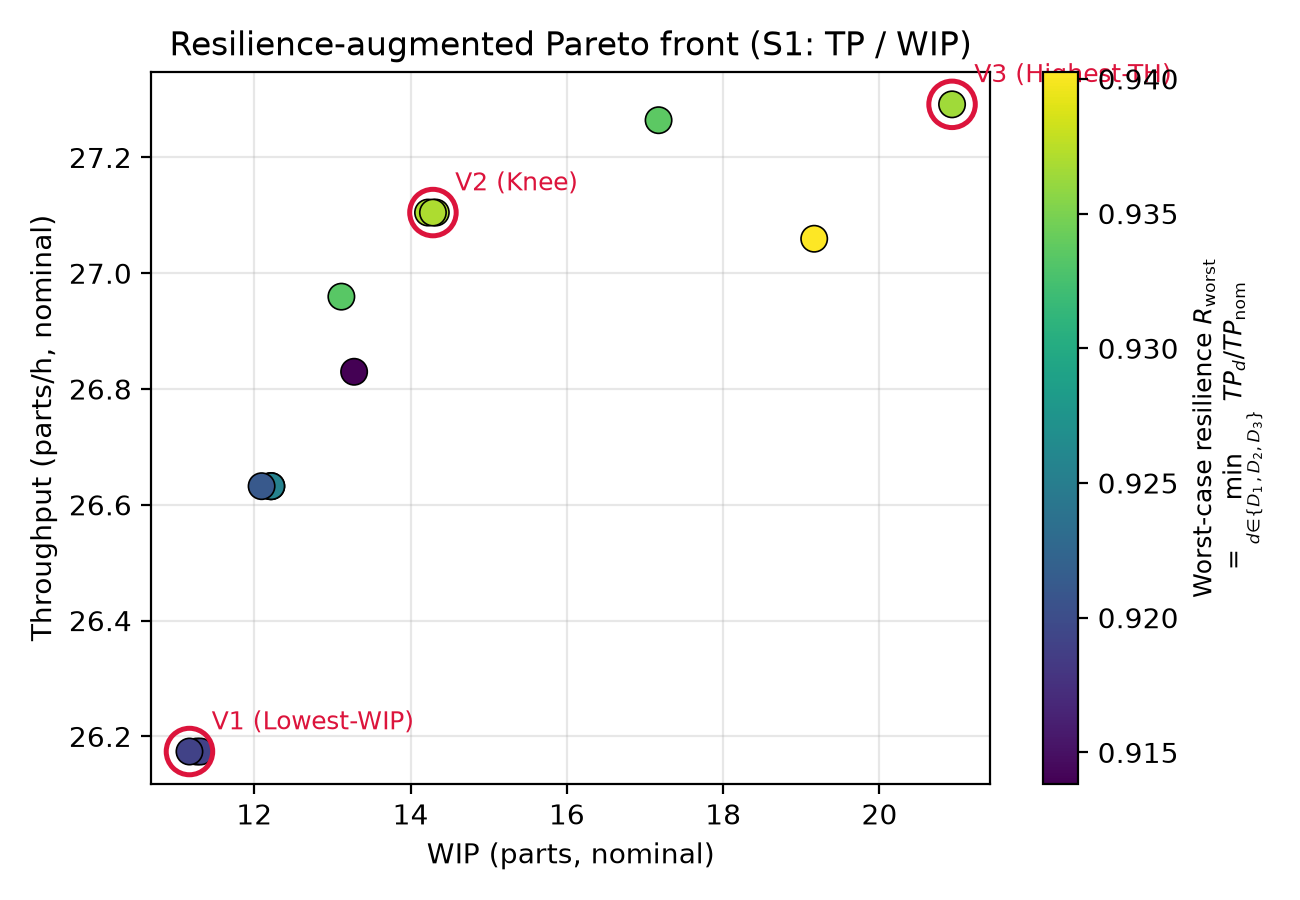
\includegraphics[width=0.7\textwidth]{figs/r1_pareto_resilience.png}                                                                      
  \caption{Performance-retention-augmented Pareto front for Scenario~S1.                                                                    
  Points are colored by their worst-case throughput-retention score                                                                         
  $R_\mathrm{worst}$ across $D_1$, $D_2$, and $D_3$. V1, V2, and V3 (the                                                                    
  three LLM-selected configurations from                                                                                                    
  Section~\ref{sec:results-moo}) are circled.}                                                                                              
  \label{fig:r1-pareto}                                                                                                                     
  \end{figure}                                                                                                                              
                                                                                                                                            
  Figure~\ref{fig:r1-matrix} disaggregates the retention score into the                                                                     
  per-scenario throughput drop for every configuration on the front,                                                                        
  sorted by $R_\mathrm{worst}$. $D_1$ and $D_2$ are the dominant sources                                                                    
  of degradation ($5.5$--$8.6$~\% drops across configurations), while                                                                       
  $D_3$ discriminates between configurations at smaller magnitudes                                                                          
  ($-0.2$ to $+1.8$~\%). Configurations with either a wide range of                                                                         
  pre-press buffering or a very deep post-press buffer best absorb the                                                                      
  Hantering feeder perturbation, whereas configurations that starve the                                                                     
  pre-press buffers suffer the largest $D_3$ drops.                                                                                         
                                                                                                                                            
  \begin{figure}[htbp]                                                                                                                      
  \centering                                                                                                                                
  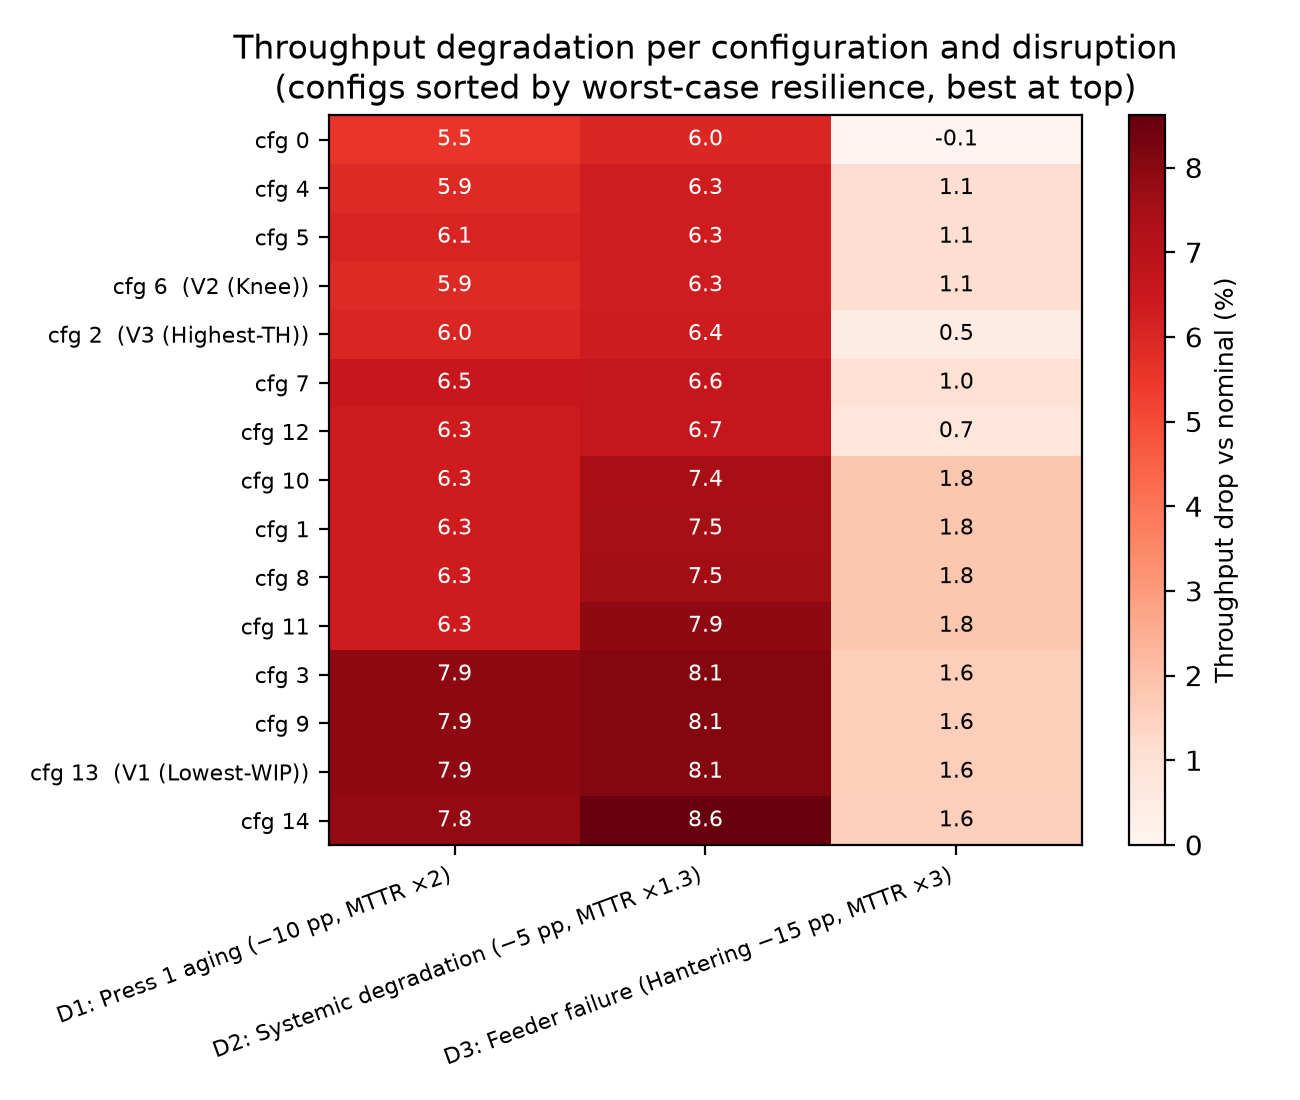
\includegraphics[width=0.8\textwidth]{figs/r1_scenario_kpi_matrix.png}                                                                    
  \caption{Throughput drop (\%) per Pareto configuration and perturbation                                                                   
  scenario. Rows are sorted from highest to lowest worst-case performance                                                                   
  retention; V1, V2, and V3 are annotated on their rows.}                                                                                   
  \label{fig:r1-matrix}                                                                                                                     
  \end{figure}                                                                                                                              
                                                                                                                                            
  \begin{figure}[htbp]                                                                                                                      
  \centering                                                
  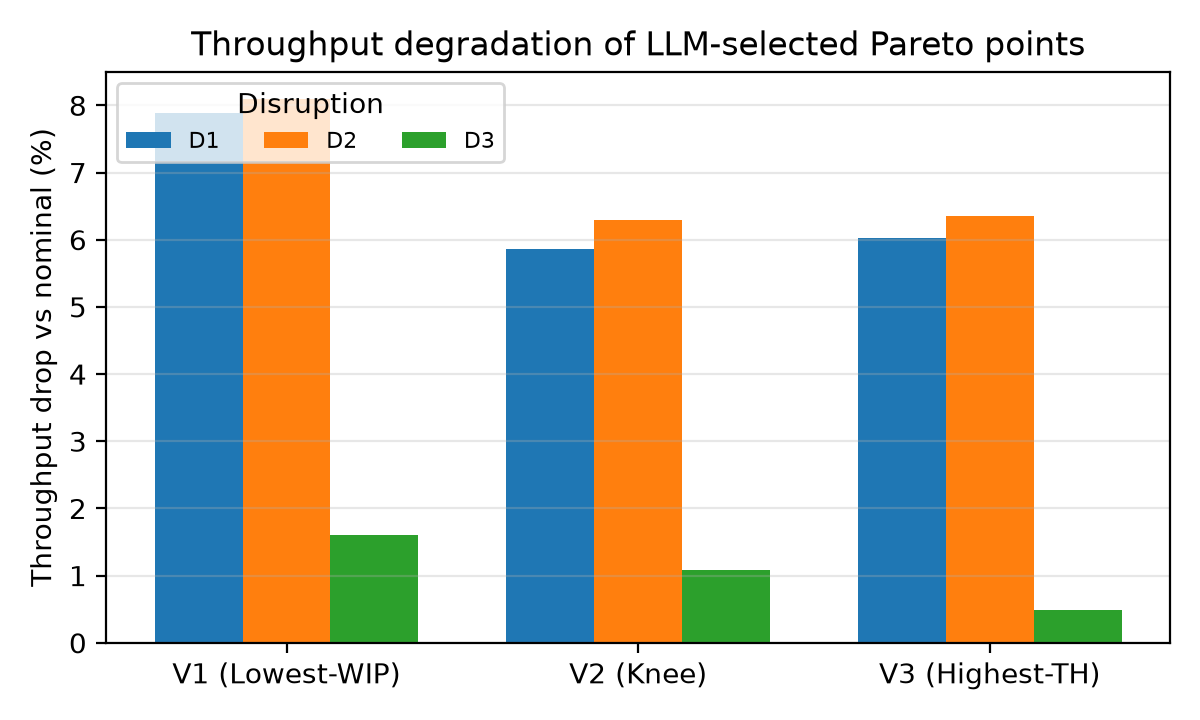
\includegraphics[width=0.6\textwidth]{figs/r1_selected_bars.png}                                                                          
  \caption{Throughput drop for V1, V2, and V3 (Table~\ref{tab:suggestions})                                                                 
  under each perturbation scenario.}                                                                                                        
  \label{fig:r1-selected}                                                                                                                   
  \end{figure}                                                                                                                              
                                                                                                                                            
  \begin{table}[htbp]                                                                                                                       
  \centering                                                                                                                                
  \caption{Performance retention of V1, V2, and V3 (the LLM-selected                                                                        
  Pareto points from Table~\ref{tab:suggestions}) under sustained                                                                           
  perturbations. Nominal TH values are means over five seeds; drops are                                                                     
  relative to the same point's nominal TH. }                                                                                            
  \label{tab:res_selected}                                                                                                                  
  \begin{tabular}{@{}l c c c c c c@{}}                                                                                                      
  \toprule                                                                                                                                  
   & \textbf{Nominal} & & \multicolumn{3}{c}{\textbf{TH drop (\%)}} & \\                                                                    
  \cmidrule(l){4-6}                                                                                                                         
  \textbf{Point} & \textbf{TH} & \textbf{Nominal WIP} & $D_1$ & $D_2$ & $D_3$ & $R_\mathrm{worst}$ \\                                       
  \midrule                                                                                                                                  
  V1 (Lowest-WIP) & 26.17 & 11.17 & 7.9 & 8.1 & 1.6 & 0.919 \\                                                                              
  V2 (Knee-point) & 27.10 & 14.29 & 5.9 & 6.3 & 1.1 & 0.937 \\                                                                              
  V3 (Highest-TH) & 27.29 & 20.93 & 6.0 & 6.4 & 0.5 & 0.936 \\                                                                              
  \bottomrule                                               
  \end{tabular}
  \end{table}

  \subsection{Scenario-conditioned bottleneck analysis}\label{sec:res-r2}                                                                   
  
  The bottleneck ranking of Section~\ref{sec:results-bn} was obtained                                                                       
  under nominal operating conditions. To ask whether the ranking itself
  is scenario-sensitive, we ran the automated SCORE analysis on the V2                                                                      
  (knee-point) buffer configuration under each of the four scenarios                                                                        
  (nominal + $D_1$ + $D_2$ + $D_3$). In each run, one machine at a time                                                                     
  received a uniform SCORE relaxation (availability $+5$~pp, MTTR                                                                           
  $\times 0.7$, PT $\times 0.9$), and its throughput gain relative to the                                                                   
  scenario-specific baseline was measured over five seeds                                                                                   
  ($4 \times 7 \times 5 = 140$ replications; the Conveyor belt, at                                                                          
  availability $100$~\% and negligible processing time, cannot be improved                                                                  
  by the relaxation and is recorded with zero gain to keep the ranking                                                                      
  complete).                                                                                                                                
                                                                                                                                            
  Figure~\ref{fig:r2-gain} shows the resulting gain matrix. The two press                                                                   
  cells dominate the response in every scenario with throughput gains                                                                       
  between $6.2$~\% and $8.8$~\%; no other machine approaches this                                                                           
  magnitude, confirming that Press cell 1 and Press cell 2 are                                                                              
  \emph{robust bottlenecks} whose alleviation should be prioritized                                                                         
  regardless of the anticipated perturbation. The ranking view in                                                                           
  Figure~\ref{fig:r2-rank} makes the same claim visually: ranks 1--2 are                                                                    
  occupied by the two press cells in all four scenarios.                                                                                    
                                                                                                                                            
  \begin{figure}[htbp]                                                                                                                      
  \centering                                                                                                                                
  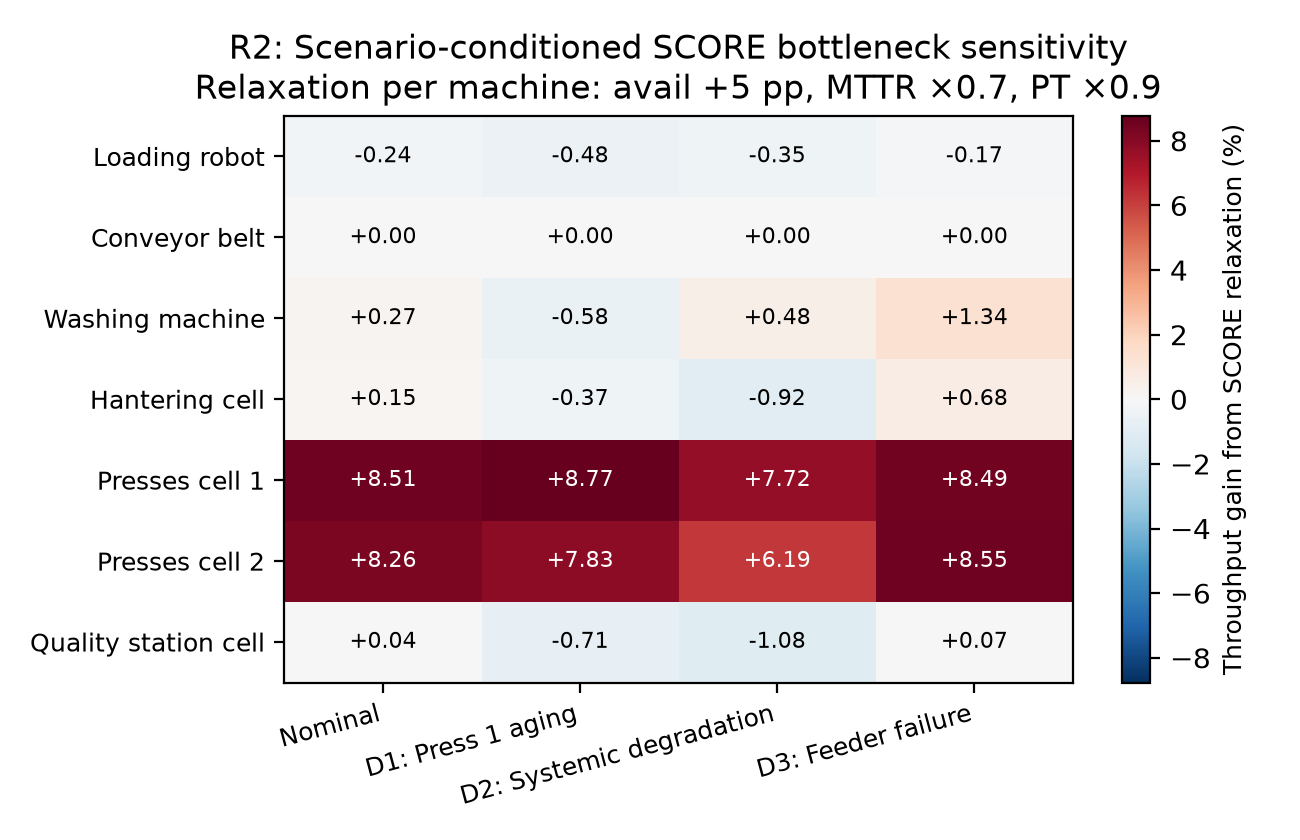
\includegraphics[width=0.8\textwidth]{figs/r2_gain_heatmap.png}                                                                           
  \caption{Throughput gain (\%) from applying a uniform SCORE relaxation                                                                    
  (availability $+5$~pp, MTTR $\times 0.7$, PT $\times 0.9$) to each                                                                        
  machine in turn, per scenario, on the V2 (knee-point) buffer                                                                              
  configuration. The two press cells dominate in every scenario.}                                                                           
  \label{fig:r2-gain}                                                                                                                       
  \end{figure}                                                                                                                              
                                                                                                                                            
  \begin{figure}[htbp]                                                                                                                      
  \centering                                                                                                                                
  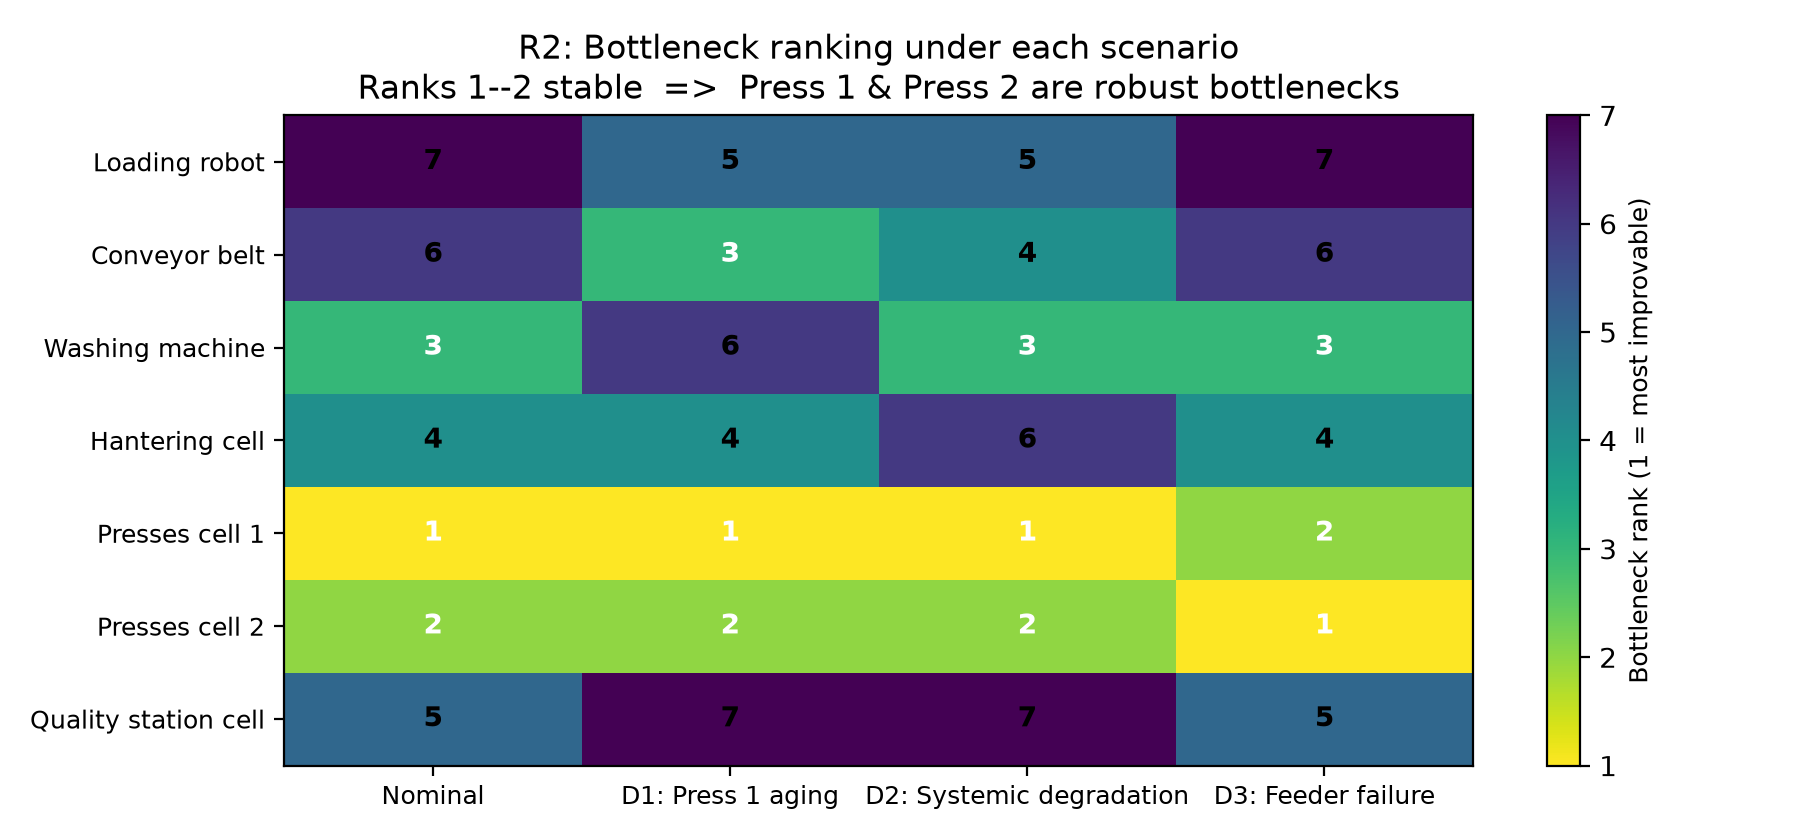
\includegraphics[width=0.9\textwidth]{figs/r2_ranking_matrix.png}                                                                         
  \caption{Bottleneck rank per scenario on the V2 (knee-point) buffer                                                                       
  configuration. Lower ranks (yellow) indicate larger improvement                                                                           
  potential; the stability of ranks 1--2 identifies the two press cells                                                                     
  as robust bottlenecks.}                                                                                                                   
  \label{fig:r2-rank}                                                                                                                       
  \end{figure}                                                                                                                              
                                                                                                                                            
  Table~\ref{tab:r2_top3} lists the top-three bottlenecks per scenario.                                                                     
  Below the two dominant presses the picture is scenario-dependent. Under                                                                   
  nominal conditions and under $D_2$ (systemic degradation), the Washing                                                                    
  machine is the next candidate for alleviation, with a modest                                                                              
  $0.27$--$0.48$~\% throughput gain. Under $D_1$ (Press~1 aging), no                                                                        
  non-press machine yields a meaningful positive gain, because the presses                                                                  
  are so much more constraining than any other station that improving                                                                       
  upstream capacity has no leverage. Under $D_3$ (feeder failure), the                                                                      
  Washing machine's alleviation gain jumps to $+1.34$~\% -- roughly five                                                                    
  times its nominal value -- because improving washing throughput allows                                                                    
  the Hantering cell to recover faster after its degraded intervals.                                                                        
  This is the kind of scenario-conditioned recommendation that a single,                                                                    
  nominal SCORE analysis cannot surface and that the framework produces                                                                     
  automatically.                                                                                                                            
                                                                                                                                            
  \begin{table}[htbp]                                                                                                                       
  \centering                                                                                                                                
  \caption{Top-three bottlenecks per scenario, ranked by throughput gain                                                                    
  from the SCORE-style relaxation on the V2 (knee-point) buffer                                                                             
  configuration. Gains are averaged over five seeds. }                                                                                     
  \label{tab:r2_top3}                                                                                                                       
  \begin{tabular}{@{}l l l l@{}}                                                                                                            
  \toprule                                                                                                                                  
  \textbf{Scenario} & \textbf{Rank 1} & \textbf{Rank 2} & \textbf{Rank 3} \\                                                                
  \midrule                                                                                                                                  
  Nominal                     & Presses cell 1 ($+8.51$\%) & Presses cell 2 ($+8.26$\%) & Washing machine ($+0.27$\%) \\                    
  $D_1$: Press 1 aging        & Presses cell 1 ($+8.77$\%) & Presses cell 2 ($+7.83$\%) & Conveyor belt ($+0.00$\%) \\                      
  $D_2$: Systemic degradation & Presses cell 1 ($+7.72$\%) & Presses cell 2 ($+6.19$\%) & Washing machine ($+0.48$\%) \\                    
  $D_3$: Feeder failure       & Presses cell 2 ($+8.55$\%) & Presses cell 1 ($+8.49$\%) & Washing machine ($+1.34$\%) \\                    
  \bottomrule                                                                                                                               
  \end{tabular}                                                                                                                             
  \end{table}                                                                                                                               
                                                                                                                                            
  \subsection{Cost of a sensitivity study}\label{sec:res-r3}                                                                                
                                                                                                                                            
  Traditional what-if analyses in industrial simulation are limited by                                                                      
  the cost of re-configuring and re-running the model for each
  perturbation scenario, which typically requires a simulation                                                                              
  specialist and hours to days per query. The framework proposed here                                                                       
  regenerates the DES, the MOEA, and the bottleneck analysis end-to-end                                                                     
  at a marginal cost on the order of a few tens of US cents and roughly                                                                     
  ten minutes per query, using the numbers reported in                                                                                      
  Table~\ref{tab:seed_metrics}. Figure~\ref{fig:r3-cost} plots                                                                              
  cumulative cost as a function of the number of what-if queries                                                                            
  answered. For a five-query sensitivity study of the type reported in                                                                      
  this section, the framework consumes on the order of USD~$1.07$ in                                                                        
  OpenAI API fees (initial $\$0.319$ from                                                                                                   
  Table~\ref{tab:seed_metrics} plus five what-if adaptations at                                                                             
  $\approx\$0.15$ each), whereas a FACTS Analyzer study performed by a                                                                      
  simulation specialist accrues on the order of USD~$9{,}000$ in                                                                            
  salaried expert time (assuming an $80$-hour initial setup and a                                                                           
  $2$-hour per-scenario rework at a loaded rate of USD~$100$/hour, both                                                                     
  conservative estimates). Time-to-answer is qualitatively similar: the                                                                     
  initial framework run completes in about $17$ minutes (992~s in                                                                           
  Table~\ref{tab:seed_metrics}) and each subsequent what-if in about                                                                        
  $8$ minutes, versus multi-day setup and multi-hour per-scenario rework                                                                    
  for a specialist-driven baseline (Figure~\ref{fig:r3-time}).                                                                              
                                                                                                                                            
  \begin{figure}[htbp]                                                                                                                      
  \centering                                                                                                                                
  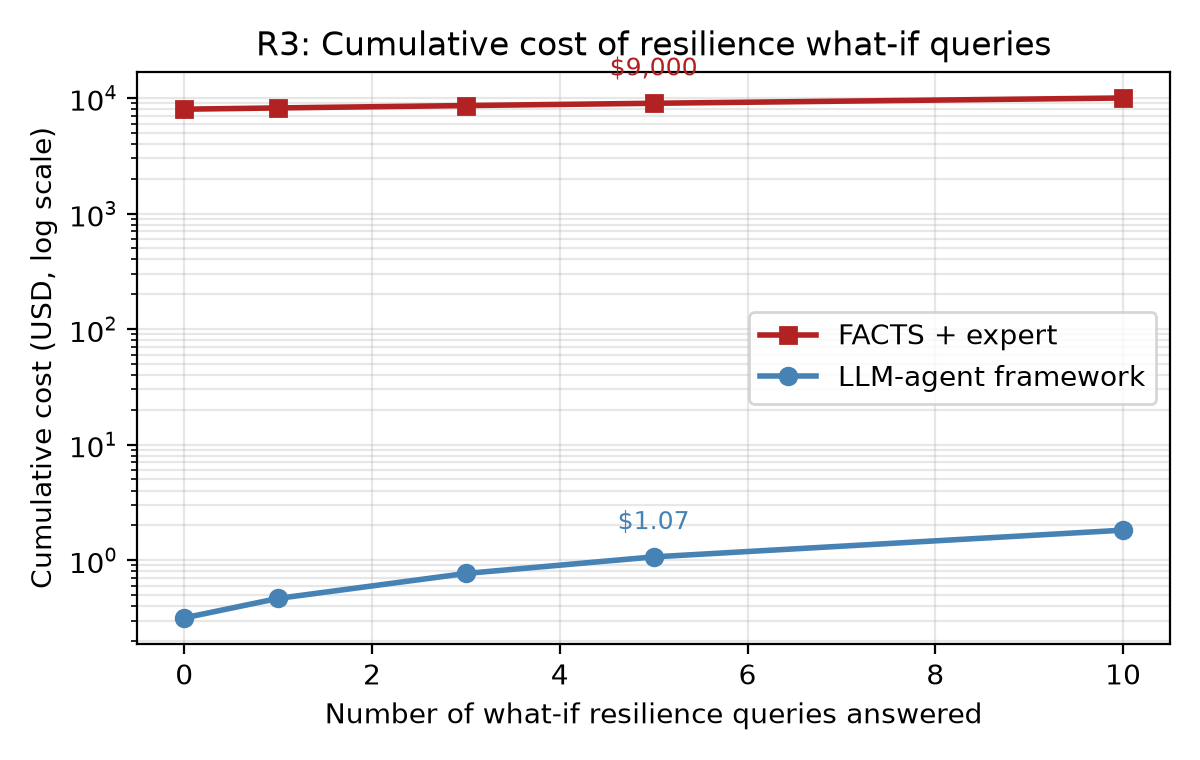
\includegraphics[width=0.7\textwidth]{figs/r3_cumulative_cost.png}                                                                        
  \caption{Cumulative cost (USD, log scale) of answering $n$ what-if                                                                        
  sensitivity queries with the proposed framework versus a                                                                                  
  FACTS-Analyzer-plus-expert baseline.}                                                                                                     
  \label{fig:r3-cost}                                                                                                                       
  \end{figure}                                                                                                                              
                                                                                                  
  \begin{figure}[htbp]                                                                                                                      
  \centering                                                                                                                                
  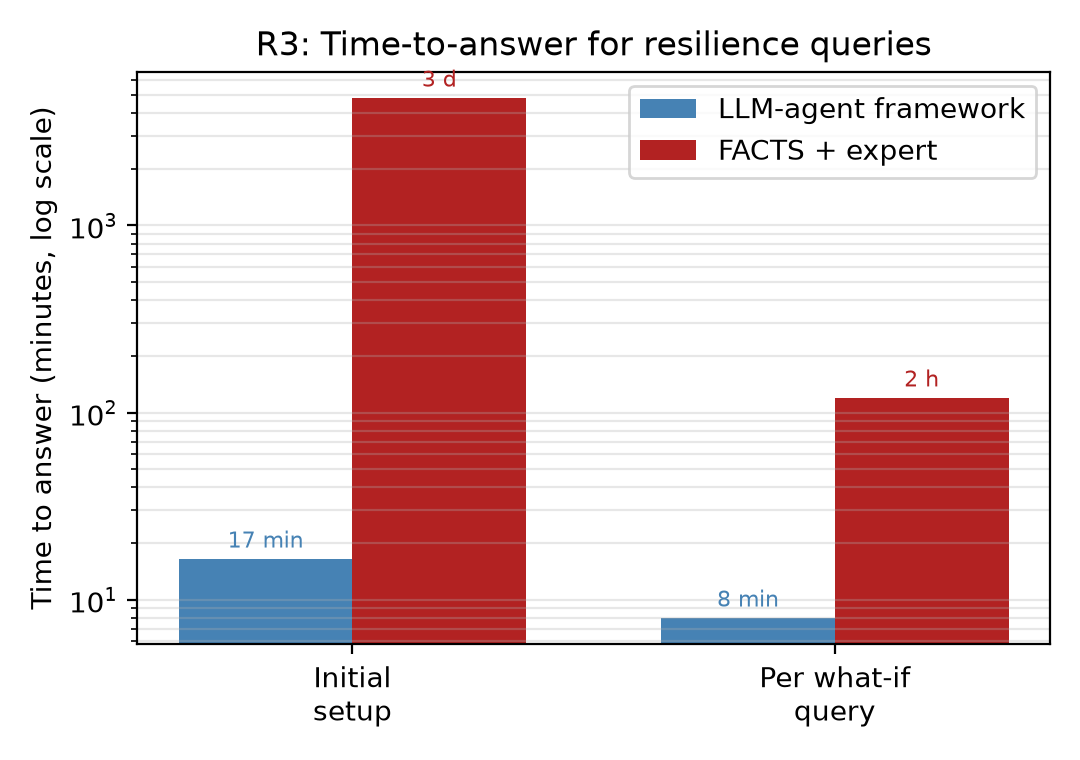
\includegraphics[width=0.55\textwidth]{figs/r3_time_to_answer.png}                                                                        
  \caption{Time-to-answer (log scale) for initial setup and for each                                                                        
  subsequent what-if sensitivity query.}                                                                                                    
  \label{fig:r3-time}                                                                                                                       
  \end{figure}                                                                                                                              
                                                                                
  Taken together, the analyses in this section show that performance                                                                        
  retention under sustained parameter perturbation is decision-relevant
  and varies across nominally Pareto-optimal configurations. The                                                                            
  scenario-conditioned bottleneck analysis further distinguishes                                                                            
  bottlenecks that remain dominant across degraded operating conditions                                                                     
  from those whose importance is scenario-dependent. These results                                                                          
  demonstrate how the framework can support one operational dimension of                                                                    
  manufacturing resilience -- performance retention -- without claiming to                                                                  
  model the full disruption-and-recovery process. We revisit the                                                                            
  implications and limitations of these findings in                                                                                         
  Section~\ref{sec:discussion}.                                                                                                             
                                                                                             
  % ======================================================================
  % 7. Discussion                                                                                                       
  % ======================================================================                                              
  \section{Discussion}\label{sec:discussion}                                                                            
                                                                                                                        
  \subsection{Where the framework performs well and where it does not}\label{sec:discussion-what}                       
                                                                                                                        
  Across the reported runs the most reliable parts of the framework are DES generation and bottleneck analysis: with the
   two blueprints active, both stages return executable artifacts on the first attempt for the great majority of seeds,
  and the automated SCORE ranking matches the FACTS Analyzer reference on the top-four alleviation actions. The MOO     
  stage is the most sensitive: it depends on the LLM selecting sensible NSGA-II hyperparameters and on the generated DES
   being fast enough to allow many candidate evaluations within a practical wall-clock budget. The SEC over-estimate
  reported in Section~\ref{sec:results-fidelity} is the most visible weakness of the current pipeline; its origin and a
  planned fix are discussed next.

  \subsection{Validity of generated KPIs}\label{sec:discussion-validity}                                                
  
  The systematic overestimate of SEC in the generated DES, on the order of 3~\% across model variants, is traced to a   
  structural difference in how idle and active states are accounted for between SimPy and FACTS Analyzer. The current
  simulation blueprint encodes a conservative interpretation that treats certain transition intervals as active; FACTS  
  treats the same intervals as idle. The discrepancy would propagate directly into any SEC-oriented Pareto front but does not affect the TH/WIP        
  scenario                                                                                                          
  or the bottleneck ranking, which is why the S1 results in Section~\ref{sec:results-moo} match the reference within
  statistical noise; a full SEC-oriented MOEA evaluation is deferred to future work (Section~\ref{sec:conclusion}). A deterministic
  post-processing step that re-classifies the affected states is a straightforward fix and is left to future work.

  \subsection{Cost characteristics for industrial use}\label{sec:discussion-cost}                                       
  
  An average full-study cost of about USD~0.32 places this framework in a qualitatively different cost regime than        
  traditional commercial simulation software, whose annual license fees are typically measured in thousands to tens of
  thousands of euros. The dominant cost driver is not the LLM calls but the simulation budget, which means that         
  optimizations of larger problems will scale primarily through compute and through improvements to the simulation
  blueprint, rather than through more expensive language models. The ablation in Section~\ref{sec:results-ablation}
  further shows that smaller models are adequate for most stages: GPT-5-mini preserves the baseline HV within
  statistical noise at roughly 43~\% of the baseline cost, whereas GPT-5-nano generates syntactically valid code but
  never returns a feasible MOO artifact. The recommended production configuration is therefore GPT-5.1 for the DES
  generation and adaptation stages, and GPT-5-mini for the visualization and evaluation stages, matching the tier
  assignment reported in Table~\ref{tab:agents}.

  \subsection{Exploratory industrial evaluation}\label{sec:discussion-industry}\label{sec:discussion-industry}                                                    
  
  To complement the quantitative evaluation, we conducted an exploratory                                                 
  evaluation with four users who interacted with the framework and
  reflected on its relevance for simulation-driven decision support. Two                                                 
  were graduate students with up to two years of experience in DES and                                                   
  optimization, while two were industrial practitioners from two large                                                   
  Swedish automotive OEMs, each with more than five years of experience                                                  
  in DES, optimization, and Pareto-based decision making. This was not                                                   
  designed as a systematic usability study; rather, its purpose was to                                                   
  obtain formative feedback from users with different levels of expertise                                                
  after they had inspected the generated model and interpreted the                                                       
  optimization and bottleneck-analysis outputs, including side-by-side                                                   
  comparisons between raw simulation results and the LLM-generated                                                       
  natural-language interpretations.                                                                                      
                                                                                                                         
  Three themes emerged consistently across the cohort. First, participants                                               
  saw value in the LLM agents for reducing the effort required to
  interpret DES and multi-objective optimization results while retaining                                                 
  human involvement in the final decision -- directly supporting the                                                     
  framework's stated aim of lowering the expertise barrier without                                                       
  displacing the practitioner. Second, the experienced practitioners                                                     
  particularly valued the simple workflow and the manual human-in-the-loop                                               
  checkpoints, which allowed intermediate outputs to be inspected for                                                    
  abnormalities before subsequent stages were triggered; one practitioner                                                
  stated that they would recommend such a framework to colleagues. This                                                  
  reinforces the design decisions on inspectability and staged HITL                                                      
  control introduced in Section~\ref{sec:framework-overview}. Third, and                                                 
  in parallel with these benefits, participants identified two concrete                                                  
  adoption requirements. On the interaction side, they requested clearer                                                 
  visualization of the production flow, an interactive UI for editing                                                    
  machine and buffer parameters without touching generated code, and                                                     
  stronger mechanisms for verifying generated models and recommendations                                                 
  before operational use. On the deployment side, trust in the framework                                                 
  was tied to data governance: using external LLM services for production                                                
  event logs was raised as a barrier that would require review under                                                     
  existing IT-security policies, with on-premises or region-hosted model                                                 
  deployments identified as a natural prerequisite for any production-line                                               
  trial.

  These observations should be read as formative rather than as evidence                                                 
  of systematic usability validation; four participants cannot support
  generalizable claims. They do, however, provide independent qualitative                                                
  support for the framework's human-in-the-loop and inspectability design                                                
  decisions, and they surface a concrete engineering agenda -- interactive                                               
  model editing, verification mechanisms, and data-governance-compliant                                                  
  deployment -- that any subsequent industrial trial will need to address.                                               
  A structured usability study across a larger and more diverse user                                                     
  population is proposed as future work in                                                                               
  Section~\ref{sec:conclusion}. 

  \subsection{Alignment with Industry~5.0}\label{sec:discussion-i5}                                                     
  
  The human-in-the-loop checkpoints, the Mermaid model visualizations, and the natural-language explanations of         
  bottleneck alleviations are the framework's most explicit alignment with the human-centric emphasis of Industry~5.0
  \citep{Toth2023,Xu2021,Turner2022hitl,Hitl2026review}. The performance-retention analysis of Section~\ref{sec:resilience} adds a second alignment with the resilience dimension of Industry~5.0 by allowing practitioners to stress-test candidate configurations and bottleneck priorities under sustained parameter perturbations. This analysis addresses performance retention rather than the complete disruption-and-recovery process.

  \subsection{Limitations}\label{sec:discussion-limits}                                                                 
  
  Four limitations should be acknowledged. First, the experiments target a single industrial case study; while Case~A is
   representative of small-to-medium serial-parallel production lines, more complex topologies (reentrant flow,
  multi-product variants) will exercise different parts of the simulation blueprint and may surface new failure modes.  
  Second, the SEC discrepancy identified in Section~\ref{sec:results-fidelity} should be resolved before the framework
  is used for energy-focused optimization. Third, the industrial reflections in Section~\ref{sec:discussion-industry}
  are informal remarks from a small number of practitioners rather than a structured usability study; a separate
  dedicated investigation of usability and non-expert accessibility remains an interesting direction for future work.
  Fourth, the analysis in Section~\ref{sec:resilience} addresses performance retention under sustained parameter perturbations, which represents only one dimension of operational resilience. It does not model transient disruptions, recovery trajectories, adaptation during recovery, or time-to-recovery. Accordingly, $R_\mathrm{worst}$ should not be interpreted as a comprehensive resilience metric. Future work should extend the framework to transient-shock experiments and time-integrated recovery measures such as the resilience triangle of \citet{Bruneau2003}, together with an appropriate steady-state assessment of the simulation horizon.

     
  % ======================================================================
  % 8. Conclusions and future work                                                                                      
  % ======================================================================                                              
  \section{Conclusions and future work}\label{sec:conclusion}

    Industrial simulation and simulation-based optimization can support complex production decisions, but their practical use remains constrained by the expertise and manual effort required to construct models, formulate optimization problems, interpret trade-offs, and translate simulation results into actionable improvement decisions. This study investigated whether these activities can instead be coordinated through an LLM-agent framework while retaining executable intermediate artifacts, quantitative validation, and human control over decision-relevant choices.

    To this end, we developed an agentic workflow that connects production data to automated discrete-event simulation, multi-objective optimization, bottleneck analysis, model adaptation, and evaluation. Rather than using the LLM itself as the simulation or optimization engine, the framework assigns language models to the generation, configuration, adaptation, and interpretation tasks while deterministic methods execute the DES, NSGA-II optimization, KPI calculations, and SCORE-based analysis. Executable blueprints constrain model generation, an inspector agent uses execution feedback to repair invalid artifacts, and human-in-the-loop checkpoints retain practitioner control over objectives, optimization settings, Pareto preferences, and model adaptations.
 
 
    Evaluation on a real automotive production line shows that this architecture can produce decision-support results close to those obtained with a commercial simulation-optimization reference. The generated DES reproduces throughput and WIP with small deviations from FACTS Analyzer, while the remaining discrepancy in specific energy consumption identifies an important boundary of the current model. For the TH/WIP optimization problem, the framework produces Pareto fronts of comparable hypervolume to the commercial reference and identifies the same dominant bottleneck-alleviation targets. The component ablation further shows that this performance does not arise from the LLM alone: the simulation and optimization blueprints substantially improve generation reliability, while execution-based inspection recovers failures that would otherwise prevent completion of the workflow. The experiments with different model tiers additionally indicate that larger language models are not required uniformly across all stages of the pipeline.

    The disruption experiments extend the evaluation beyond nominal operating conditions. Pareto-optimal configurations differ in their ability to retain throughput under sustained equipment and reliability degradation, showing that nominal TH/WIP performance alone does not characterize their behavior under perturbed conditions. The scenario-conditioned bottleneck analysis further distinguishes bottlenecks that remain dominant across degraded operating conditions from those whose importance depends on the disruption scenario. These experiments address performance retention as one operational component of resilience rather than the complete disruption-and-recovery process.

    Taken together, the results suggest that the main opportunity for LLMs in simulation-driven industrial decision support is not to replace simulation, optimization, or engineering expertise, but to reduce the manual integration effort between them. The framework provides a way to translate production data and practitioner intent into executable and inspectable simulation-analysis workflows, while keeping numerical computation deterministic and preference-sensitive decisions visible to the human user. At the same time, the SEC discrepancy and the observed generation failures demonstrate that executable code alone is not evidence of engineering validity; generated models and their decision outputs must still be validated against domain knowledge and trusted references.

    Future work should therefore focus on both broader validation and stronger safeguards. The framework should be evaluated on production systems with more complex topologies, including reentrant flows and multi-product environments, and the energy-accounting discrepancy should be resolved before sustainability-oriented optimization is used operationally. Resilience analysis should be extended from sustained parameter perturbations to transient disruptions and recovery trajectories. The bottleneck agent could also be extended from individual alleviation actions to combinations of interacting improvements. Finally, structured studies with industrial practitioners are needed to quantify usability, trust, and the extent to which the proposed human-in-the-loop design can reduce the expertise barrier to simulation-driven decision support.

  % ======================================================================                                              
  % Declarations
  % ======================================================================                                              
  \section*{Declaration of competing interest}                                                                          
  The authors declare that they have no known competing financial interests or personal relationships that could have   
  appeared to influence the work reported in this paper.                                                                
                                                                                                                        
  \section*{Declaration of generative AI use in the writing process}                                                    
  During the preparation of this work, the authors partially used Claude (Anthropic) to assist with copy-editing and formatting of individual paragraphs. After using these tools, the authors reviewed and edited the content as needed and take full responsibility for the content of the publication. This declaration is distinct from the LLM-based framework that is the subject of the research itself, whose full model tier, prompts, and code are documented in Sections~\ref{sec:framework} and~\ref{sec:results-ablation}.

  \section*{Data availability}\label{sec:data-availability}                                                             
The source code, the three blueprints, an anonymized version of the Case~A event log, and the scripts used to         
  reproduce every table and figure in this paper are available at \url{https://github.com/Peggy4444/LLM-DES-MOO-Public}.
   An interactive demonstration of the framework is hosted at \url{https://llm-des-moo.streamlit.app/}. On acceptance, a
   frozen release of the repository will be archived on Zenodo and the corresponding DOI added to this section.     .                          
                                                                                                                        
  \section*{Acknowledgments}                                                                                            
  The authors thank Mats Gustafsson and Matias Urenda Moris for valuable feedback during the project, and colleagues at Uppsala University and
  the host company for the discussions that informed this work.       
  This study was partially funded by Sweden’s Innovation Agency (Vinnova) through the AI-COMPETE project (grant number 2025-01066).
  The computations were enabled by resources in project [NAISS 2026/4-892] provided by the National Academic Infrastructure for Supercomputing in Sweden (NAISS) at UPPMAX, funded by the Swedish Research Council through grant agreement no. 2022-06725.
                                                            
  % Print CRediT contribution statement (generated from \credit{...} above).                                            
  \printcredits                                             
                                                                                                                        
  % ----------------------------------------------------------------------                                              
  % Bibliography                                                                                                        
  % ----------------------------------------------------------------------                                              
  \bibliographystyle{cas-model2-names}                                                                                  
  \bibliography{references}                                                                                             
                                                                                                                        
  \end{document}                     